\documentclass[output=paper,draft,draftmode,colorlinks,citecolor=brown]{langscibook}
\ChapterDOI{10.5281/zenodo.7353621}
%updated February 20, 2022
\title{Privation and Negation: Semantic change in the negative domains of three Australian (Pama-Nyungan) language groups}
\shorttitlerunninghead{Semantic change in three Australian language groups}
\author{Joshua Phillips\affiliation{Yale University}} 

\iffalse
\begin{comment}
\newglossary*{lang}{Language index}
\newglossary*{gloss}{List of abbreviations}
\makeglossaries
% abbreviations:
\newglossaryentry{rit}{
	name = \texttt{rit} ,
	description = Ritharrŋu (Pama-Nyungan: Yolŋu (Yaku)),
	type=lang,	}
\newglossaryentry{jay}{
	name = \texttt{jay} ,
	description = Yan-nhaŋu (Pama-Nyungan: Yolŋu (Nhaŋu)),
	type=lang,	}
\newglossaryentry{djr}{
	name = \texttt{djr} ,
	description = Djambarrpuyŋu (Pama-Nyungan: Yolŋu (Dhuwal)),
	type=lang,	}
\newglossaryentry{guf}{
	name = \texttt{guf} ,
	description = Gupapuyŋu (Pama-Nyungan: Yolŋu (Dhuwala)),
	type=lang,	}
\newglossaryentry{yil}{
	name = \texttt{yil} ,
	description =  Bularnu (Pama-Nyungan: Warluwaric),
	type=lang,	}
\newglossaryentry{wrb}{
	name = \texttt{wrb} ,
	description =  Warluwarra (Pama-Nyungan: Warluwaric),
	type=lang,	}
\newglossaryentry{dhg}{
	name = \texttt{dhg} ,
	description = Wangurri (Pama-Nyungan: Yolŋu (Dhaŋu)),
	type=lang,	}
\newglossaryentry{nna}{
	name = \texttt{nna} ,
	description = Nyangumarta (Pama-Nyungan: Marrngu),
	type=lang,	}
\newglossaryentry{dif}{
	name = \texttt{dif} ,
	description = Diyari (Pama-Nyungan: Karnic),
	type=lang,	}
\newglossaryentry{mem}{
	name = \texttt{mem} ,
	description = Mangala (Pama-Nyungan: Marrngu),
	type=lang,	}
\newglossaryentry{aer}{
	name = \texttt{aer} ,
	description = Upper Arrernte (Pama-Nyungan: Arandic),
	type=lang,	}
\newglossaryentry{mao}{
	name = \texttt{mao} ,
	description = Maori (Polynesian; New Zealand),
	type=lang,	}
\newglossaryentry{mec}{
	name = \texttt{mec} ,
	description = Marra (?Arnhem: Marran),
	type=lang,	}
\newglossaryentry{nid}{
	name = \texttt{nid} ,
	description = Marra (?Arnhem: East),
	type=lang,	}
\newglossaryentry{wgu}{
	name = \texttt{wgu} ,
	description = Wirangu (Pama-Nyungan: Thura-Yura),
	type=lang,	}
\newglossaryentry{wga}{
	name = \texttt{wga} ,
	description = Wakaya (Pama-Nyungan: Warluwaric),
	type=lang,	}
\newglossaryentry{bcj}{
	name = \texttt{bcj} ,
	description = Bardi (Pama-Nyungan: Nyulnyulan),
	type=lang,	}
\newglossaryentry{wyb}{
	name = \texttt{wyb} ,
	description = Ngiyambaa (Pama-Nyungan: Wiradhuric),
	type=lang,	}
\newglossaryentry{pjt}{
	name = \texttt{pjt} ,
	description = Pitjantjatjara (Pama-Nyungan: Wati),
	type=lang,	}
\newglossaryentry{kdd}{
	name = \texttt{kdd} ,
	description = Yankunytjatjara (Pama-Nyungan: Wati),
	type=lang,	}
\newglossaryentry{wrg}{
	name = \texttt{wrg} ,
	description = Warrongo (Pama-Nyungan: Maric),
	type=lang,	}
\newglossaryentry{bym}{
	name = \texttt{bym} ,
	description = Bidjara (Pama-Nyungan: Maric),
	type=lang,	}
\newglossaryentry{dbl}{
	name = \texttt{dbl} ,
	description = Dyirbal (Pama-Nyungan: Dyirbalic),
	type=lang,	}
\newglossaryentry{gbb}{
	name = \texttt{gbb} ,
	description = Kaytetye (Pama-Nyungan: Arandic),
	type=lang,	}
\newglossaryentry{bjb}{
	name = \texttt{bjb} ,
	description = Barngarla (Pama-Nyungan: Thura-Yura),
	type=lang,	}
\newglossaryentry{adt}{
	name = \texttt{adt} ,
	description = Adnyamathanha (Pama-Nyungan: Thura-Yura),
	type=lang,	}
\newglossaryentry{gvy}{
	name = \texttt{gvy} ,
	description = Kuyani (Pama-Nyungan: Thura-Yura),
	type=lang,	}
\newglossaryentry{nnv}{
	name = \texttt{nnv} ,
	description = Nukunu (Pama-Nyungan: Thura-Yura),
	type=lang,	}
\newglossaryentry{nwo}{
	name = \texttt{nwo} ,
	description = Nauo (Pama-Nyungan: Thura-Yura),
	type=lang,	}
\newglossaryentry{zku}{
	name = \texttt{zku} ,
	description = Kaurna (Pama-Nyungan: Thura-Yura),
	type=lang,	}
\newglossaryentry{nyt}{
	name = \texttt{nyt} ,
	description = Nyawaygi (Pama-Nyungan: Dyirbalic),
	type=lang,	}
\newglossaryentry{kgs}{
	name = \texttt{kgs} ,
	description = Gumbaynggir (Pama-Nyungan: Southeast NSW),
	type=lang,	}
\newglossaryentry{zmu}{
	name = \texttt{zmu} ,
	description = Muruwari (Pama-Nyungan: Southeast NSW),
	type=lang,	}
\newglossaryentry{ktd}{
	name = \texttt{ktd} ,
	description = Kokata (Pama-Nyungan: Wati),
	type=lang,	}
\newglossaryentry{priv}{
	name = \textsc{priv} ,
	description = privative case , 
	type = gloss , }
\newglossaryentry{sn}{
	name = \textsc{SN} ,
	description = standard negation\slash negator, 
	type = gloss , }
\newglossaryentry{NEC}{
	name = \textsc{NEC} ,
	description = Negative Existential Cycle,
	type = gloss , }
\newglossaryentry{NP}{
	name = \textsc{NP} ,
	description = noun phrase,
	type = gloss , }
\newglossaryentry{proh}{
	name = \textsc{proh} ,
	description = prohibitive,
	type = gloss , }
\newglossaryentry{recp}{
	name = \textsc{recp} ,
	description = reciprocal,
	type = gloss , }
\newglossaryentry{neg}{
	name = \textsc{neg} ,
	description = negator,
	type = gloss , }
\newglossaryentry{all}{
	name = \textsc{all} ,
	description = allative case,
	type = gloss , }
\newglossaryentry{abl}{
	name = \textsc{abl} ,
	description = ablative case,
	type = gloss , }
\newglossaryentry{acc}{
	name = \textsc{acc} ,
	description = accusative case,
	type = gloss , }
\newglossaryentry{nom}{
	name = \textsc{nom} ,
	description = nominative case,
	type = gloss , }
\newglossaryentry{prs}{
	name = \textsc{prs} ,
	description = present tense,
	type = gloss , }
\newglossaryentry{erg}{
	name = \textsc{erg} ,
	description = ergative case,
	type = gloss , }
\newglossaryentry{dp}{
	name = \textsc{dp} ,
	description = ``discourse clitic'' \citep{McLellan1992},
	type = gloss , }
\newglossaryentry{ints}{
	name = \textsc{ints} ,
	description = intensifier,
	type = gloss , }
\newglossaryentry{neg.ex}{
	name = \textsc{neg.ex} ,
	description = negative existential\slash quantifier,
	type = gloss , }
\newglossaryentry{red}{
	name = \textsc{red} ,
	description = reduplicant,
	type = gloss , }
\newglossaryentry{neg.quant}{
	name = \textsc{neg.quant} ,
	description = negative quantifier (existential) $\nexists$,
	type = gloss , }
\newglossaryentry{com}{
	name = \textsc{com} ,
	description = comitative case,
	type = gloss , }
\newglossaryentry{prop}{
	name = \textsc{prop} ,
	description = proprietive case,
	type = gloss , }
\newglossaryentry{perl}{
	name = \textsc{perl} ,
	description = perlative case,
	type = gloss , }
\newglossaryentry{inch}{
	name = \textsc{inch} ,
	description = inchoative,
	type = gloss , }
\newglossaryentry{seq}{
	name = \textsc{seq} ,
	description = sequential,
	type = gloss , }
\newglossaryentry{abs}{
	name = \textsc{abs} ,
	description = absolutive case,
	type = gloss , }
\newglossaryentry{prom}{
	name = \textsc{prom} ,
	description = prominence marker ($\approx$ focus),
	type = gloss , }
\newglossaryentry{nmlz}{
	name = \textsc{nmlz} ,
	description = nominaliser (derivation),
	type = gloss , }
\newglossaryentry{anaph}{
	name = \textsc{anaph} ,
	description = ``anaphoric reference'' \citep{McLellan1992},
	type = gloss , }
\newglossaryentry{foc}{
	name = \textsc{foc} ,
	description = focus marker
	type = gloss , }
\newglossaryentry{loc}{
	name = \textsc{loc} ,
	description = locative case,
	type = gloss , }
\newglossaryentry{per}{
	name = \textsc{per} ,
	description = pergressive case,
	type = gloss , }
\newglossaryentry{excl}{
	name = \textsc{excl} ,
	description = exclusive (1ns-pronoun),
	type = gloss , }
\newglossaryentry{pst}{
	name = \textsc{pst} ,
	description = past tense,
	type = gloss , }
\newglossaryentry{incl}{
	name = \textsc{incl} ,
	description = inclusive (1ns-pronoun),
	type = gloss , }
\newglossaryentry{dist}{
	name = \textsc{dist} ,
	description = distal (demonstrative),
	type = gloss , }
\newglossaryentry{prox}{
	name = \textsc{prox} ,
	description = proximal (demonstrative),
	type = gloss , }
\newglossaryentry{med}{
	name = \textsc{med} ,
	description = medial (demonstrative),
	type = gloss , }
\newglossaryentry{texd}{
	name = \textsc{texd} ,
	description = ``textual deictic'' \citep{Wilkinson1991} (demonstrative),
	type = gloss , }
\newglossaryentry{obl}{
	name = \textsc{obl} ,
	description = oblique case,
	type = gloss , }
\newglossaryentry{dat}{
	name = \textsc{dat} ,
	description = dative case,
	type = gloss , }
\newglossaryentry{ds}{
	name = \textsc{ds} ,
	description = different subject (subordinate clause),
	type = gloss , }
\newglossaryentry{ipfv}{
	name = \textsc{ipfv} ,
	description = imperfective (aspect),
	type = gloss , }
\newglossaryentry{imp}{
	name = \textsc{imp} ,
	description = imperative,
	type = gloss , }
\newglossaryentry{pfv}{
	name = \textsc{pfv} ,
	description = perfective (aspect),
	type = gloss , }
\newglossaryentry{fut}{
	name = \textsc{fut} ,
	description = future (tense),
	type = gloss , }
\end{comment}
\fi

\abstract{On the basis of comparative data in three Pama-Nyungan subfamilies (Thura-Yura, Yolŋu Matha and Arandic), this chapter brings comparative data from the Aboriginal languages of Australia to bear on the Negative Existential Cycle (NEC, see \citealt{Croft1991}, Veselinova this volume a.o.). I propose a formal semantic analysis of the Cycle, where the, a grammatical category described in many Australian languages (e.g. \citealt{Dixon2002a}), is taken to realise the semantics of a negative existential. Diachronically, I show that erstwhile privatives generalise into sentential negators: an instantiation of the NEC.

\textbf{Keywords:} negation, privatives, existentials, semantic change, Australian languages, quanti ication}

\IfFileExists{../localcommands.tex}{
   \usepackage{langsci-optional}
\usepackage{langsci-gb4e}
\usepackage{langsci-lgr}

\usepackage{listings}
\lstset{basicstyle=\ttfamily,tabsize=2,breaklines=true}

%added by author
% \usepackage{tipa}
\usepackage{multirow}
\graphicspath{{figures/}}
\usepackage{langsci-branding}

   
\newcommand{\sent}{\enumsentence}
\newcommand{\sents}{\eenumsentence}
\let\citeasnoun\citet

\renewcommand{\lsCoverTitleFont}[1]{\sffamily\addfontfeatures{Scale=MatchUppercase}\fontsize{44pt}{16mm}\selectfont #1}
  
   %% hyphenation points for line breaks
%% Normally, automatic hyphenation in LaTeX is very good
%% If a word is mis-hyphenated, add it to this file
%%
%% add information to TeX file before \begin{document} with:
%% %% hyphenation points for line breaks
%% Normally, automatic hyphenation in LaTeX is very good
%% If a word is mis-hyphenated, add it to this file
%%
%% add information to TeX file before \begin{document} with:
%% %% hyphenation points for line breaks
%% Normally, automatic hyphenation in LaTeX is very good
%% If a word is mis-hyphenated, add it to this file
%%
%% add information to TeX file before \begin{document} with:
%% \include{localhyphenation}
\hyphenation{
affri-ca-te
affri-ca-tes
an-no-tated
com-ple-ments
com-po-si-tio-na-li-ty
non-com-po-si-tio-na-li-ty
Gon-zá-lez
out-side
Ri-chárd
se-man-tics
STREU-SLE
Tie-de-mann
}
\hyphenation{
affri-ca-te
affri-ca-tes
an-no-tated
com-ple-ments
com-po-si-tio-na-li-ty
non-com-po-si-tio-na-li-ty
Gon-zá-lez
out-side
Ri-chárd
se-man-tics
STREU-SLE
Tie-de-mann
}
\hyphenation{
affri-ca-te
affri-ca-tes
an-no-tated
com-ple-ments
com-po-si-tio-na-li-ty
non-com-po-si-tio-na-li-ty
Gon-zá-lez
out-side
Ri-chárd
se-man-tics
STREU-SLE
Tie-de-mann
}
   \togglepaper[1]%%chapternumber
}{}


\begin{document}


\AffiliationsWithoutIndexing{}
\maketitle

\section{Introduction}\label{sec:austr-1}

This chapter brings the observations of the ``negative existential cycle''
(see \citealt{Croft1991}, \citealt{Veselinova2013,Veselinova2016}, this
volume among others) to bear in the context of the Aboriginal languages of
Australia. The Australian language ecology is a fertile area for
comparative typological work, given its striking linguistic diversity and
small, non-sedentary, frequently exogamous populations \citep{Bowern2010}.
Some 90\% ($N\approx290$) of the languages spoken on the Australian
mainland have been reconstructed to the Pama-Nyungan\il{Pama-Nyungan|(} family \parencites(see
also)(){OVV1966}{Wurm1972}{BowernAtkinson2012}, with a common ancestor spoken in Northern Australia almost 6,000 years before present \citep{BouckaertBowern2018}.

Taking the negative domains of three Pama-Nyungan subgroups as an empirical
testing ground, this chapter describes the relationship between
so-called ``standard'' (SN) and ``existential'' negation in an
investigation of predictions made by a postulated cyclic change: the
Negative Existential Cycle (NEC). Here, explicit markers of existential 
negation%
    \footnote{For the purposes of this paper, similarly to others in the current volume, ``existential negation'' is understood as a linguistic strategy for predicating the \textit{absence} of some entity at a certain location (adapting from Creissels' \citeyearpar[2]{Creissels2014} typology of existential constructions, consonant with the approach taken in \citealp[139]{Veselinova2013}. McNally also points out the relevance of ``noncanonical sentence types'', distinguished syntactically or lexically, serving to ``introduce the presence or existence of some individual(s)'' \citeyearpar[210]{McNally2016}. See also \citealt{Freeze1992} for an analysis that explicitly relates existential to \textsc{locative} and \textsc{possessive} predications.} 
%
emerge (stage $A\to B$), encroach into the semantic domain of an erstwhile general negative marker (stage $B\to C$), and finally displace the latter, becoming a standard negation marker without the formal or functional features of an existential negator (stage $C\to A$; see \citealt{Croft1991,Veselinova2016} a.o.) The Pama-Nyungan data provided here give further evidence for the cross-linguistic validity of the NEC, although, we will also see evidence of contact-induced change in the negative domains of some languages which are not clearly captured by the Cycle.

%\begin{wrapfigure}{r}{.595\textwidth}
\begin{figure}
	\begin{tikzpicture}[scale=0.25]\footnotesize
	\tikzstyle{every node}+=[inner sep=0pt]
	\draw [black] (23.6,-7.9) circle (3);
	\draw (23.6,-7.9) node[rectangle split,rectangle split parts=2] {\textbf{A}\nodepart{second} $\neg\phi/\neg\exists x$};
	\draw [black] (13.2,-24) circle (3);
	\draw (13.2,-24) node[rectangle split,rectangle split parts=2] {\textbf{C}\nodepart{second} $\nexists\phi/\nexists x$};
	\draw [black] (33.6,-24) circle (3);
	\draw (33.6,-24) node[rectangle split,rectangle split parts=2] {\textbf{B}\nodepart{second} $\neg\phi/\nexists x$};
	\draw [black] (26.574,-8.22) arc (76.02264:-12.33232:10.957);
	\fill [black] (34.63,-21.19) -- (35.29,-20.52) -- (34.31,-20.3);
	\draw [black] (12.391,-21.12) arc (-171.74775:-253.97416:11.563);
	\fill [black] (20.64,-8.35) -- (19.74,-8.09) -- (20.01,-9.05);
	\draw [black] (31.586,-26.214) arc (-49.16439:-130.83561:12.519);
	\fill [black] (15.21,-26.21) -- (15.49,-27.12) -- (16.15,-26.36);
	\end{tikzpicture}
	
	\caption{The ``Negative Existential cycle'' -- a typology of standard and existential negation according to the analyticity of these markers (\citealt{Croft1991}, see also \citealt{Veselinova2016}.) Standard negators $\neg$ are used to negate both verbal $\phi$ and existential $\exists$ predicates in stage A, a suppletive ``negative existential'' $\nexists$ arises in stage B and this marker comes to mark standard negation in stage C. ``Transitional'' stages are assumed to occur between each of the labelled stages.}\label{fig:austr-Croft-cycle}
\end{figure}

This chapter is organised as follows: \sectref{sec:austr-2} provides an
overview of typological generalisations that can be made of negation
marking in Australian languages with particular attention paid to the
semantics of the category of the so-called ``privative case.''
\sectref{sec:austr-3} investigates evidence of change, replacement and
renewal of negative markers in the Thura-Yura language group of South
Australia. \sectref{sec:austr-4} compares the negative domains of three
Yolŋu languages, particularly evidence of expansion in the domain of
privative marking in a number of varieties. \sectref{sec:austr-5}
describes standard negation in Upper Arrernte, situating arguments made
elsewhere in the literature \citep[particularly][]{Henderson2013} that,
in this language (and related Arandic varieties), synchronic SN
strategies are a result of reanalysis of an erstwhile nominal suffix.
Ultimately, a primary upshot of this comparative work trades on an
insight, only briefly discussed in work on the NEC
\parencite[e.g.][17]{Croft1991}, that this process (at least insofar as
it is actualised in these Australian languages) can largely be
understood and predicted with reference to existing work on semantic
change (sc. diachronic developments in the meaning of a given
lexical item) and work that formally seeks to generalise over
grammaticalisation pathways and cycles 
\parencites(e.g.)(){Deo2015}{Deo2015a}{Deo2018}.%
%
\footnote{See also the distinction drawn between ``functional'' and ``formal'' cycles as applied to the Jespersen's cycle in \citet{AhernClark2017}.} This is discussed in \sectref{sec:austr-6}.

\section{Negation and Australia: a typological snapshot}\label{sec:austr-2}
\begin{figure}%{.5\textwidth}
	\includegraphics[scale=.5]{figures/YolTYAr-leg}
	\caption{Subgrouping of Australian languages. Pama-Nyungan family is tan, with Yolŋu subgroup given in in ochre, Arandic in purple and Thura-Yura in blue (Western\slash Nangga varieties) and green (Eastern varieties.) Map adapted from \citet[xxviii]{Dixon2002a}, colourised by author.}
\end{figure}\noindent

Strategies that natural languages deploy to mark negation have long attracted the attention of philosophers and linguists (see \citealt{Horn1989} for a comprehensive investigation of these questions). More recent work (e.g. \citealt{Miestamo2005} a.o.) seeks to propose a typology for the behavior of ``standard negation'' marking strategies across a sample of world languages (including 40 Australian varieties.) \textit{Standard negation} (SN) is understood as those language-specific mechanisms whose function is the inversion of the truth value of a proposition associated with a given (declarative) clause. Drawing a distinction between SN and ``special negation'' is warranted in view of the empirical fact that many languages have distinct formal mechanisms for the negation of nonverbal (e.g. copular, existential) predications, imperatives and other types of ``subclausal'' negation \citep{Miestamo2007,HornWansing2017,Veselinova2013,AuweraLejeune2005}.

Some 300 Australian languages have been reconstructed to a single family, Pama-Nyungan, spoken across Australia except for some regions in the north of the continent. The most recent common ancestor of these languages is esimated to have been spoken roughly five to six thousand years \textsc{BP} (a similar timedepth to Indo-European, see \citealt[742]{BouckaertBowern2018}). Many of these languages remain underdescribed, and consequently, typological and comparative work detailing the expression of negation across Australian languages is underdeveloped. Exceptions to this include \citealp{Dixon2002a} and \citeauthor{PhillipsFCb} (forthcoming): surveys that have turned up some generalisations about the formal and functional expression of negation in these languages. Based on the insights of these works, we might divide the ``negative semantic space'' so to distinguish four macro-categories of negator: (1) negative imperatives\slash prohibitives, (2) clausal\slash standard negators and (3) nominal negators, including specialised negative existentials and a commonly occurring ``privative'' category, and (4) negative interjections. There is a substantial amount of variation in the formal exponence of each of these functions, some varieties distinguishing all four categories  (e.g. Bidjara [bym]), some with a single syncretic marker for all four (e.g. Dyirbal [dbl], according to \citealp[84--table 3.3]{Dixon2002a}). 

\hspace*{-3pt}An exceptionful (but otherwise fairly robust) formal tendency across Australian languages is for clausal negation to be marked with a particle pre-verbally and for privative case to be encoded as a nominal suffix. We will explore the implications of this generalisation and its exceptions below. The remainder of this section constitutes a brief survey the exponence of negation strategies in Australian languages, partially summarising insights from \citeauthor{PhillipsFCb} (forthcoming).

\subsection{``Standard'' negation}

This section briefly provides some generalisations about clausal negation strategies in Australian languages. For a more comprehensive discussion of exceptions and significant interactions between SN and other aspects of the verbal complex in Australian languages, the reader is referred to \citeauthor{PhillipsFCb} (forthcoming).

\citet[82]{Dixon2002a} claims that ``almost every Australian language marks
`not' by a non-inflecting particle which goes before the verb.'' He notes
that this generalisation extends also to the most synthetic
non-Pama-Nyungan languages spoken in the north of the continent. Negation
in the Arandic subgroup of Pama-Nyungan, which provides a major exception
to this formal generalisation, and is particularly relevant for current
purposes, is discussed in more detail in \sectref{sec:austr-5}. The data
from Ngiyambaa ([wyb] Pama-Nyungan: Wiradhuric) below clearly demonstrate
this generalisation with the preverbal SN particle \textit{waŋaːy}, which
has scope over the entire sentence in \REF{ex:austr-Ngiyambaa-wake-a} and just the second predicate in \REF{ex:austr-Ngiyambaa-wake-b}.
\begin{exe}\ex\label{sn-wyb} Preverbal standard negation in Ngiyambaa \citep[239]{Donaldson1980}
    \begin{xlist}
\ex\label{ex:austr-Ngiyambaa-wake-a}
    \gll \textbf{Waŋaːy} yiŋgalaː-dhi\textdblhyphen dju\textdblhyphen na girimiyi-la.\\
\textsc{\textbf{neg}} same-\textsc{circ}\textdblhyphen 1.\textsc{nom}\textdblhyphen3.\textsc{abs} wake\textsc{.pst-then}\\
\glt `It wasn't because of that I woke her then.'
\ex\label{ex:austr-Ngiyambaa-wake-b}
    \gll Yiŋgalaː-dhi\textdblhyphen dju\textdblhyphen na \textbf{waŋaːy} girimiyi-la.\\
same-\textsc{circ}\textdblhyphen 1.\textsc{nom}\textdblhyphen3.\textsc{abs} \textsc{\textbf{neg}} wake\textsc{.pst-then}\\
\glt `Because of that I didn't wake her then.'
    \end{xlist}\end{exe}

\subsection{The ``privative case'' and existential predications}\label{sec:austr-2.2}

The privative case (\textsc{priv}) is a very robustly attested category in
Australian languages.\footnote{Morphological cases with similar
semantics are referred to as \textit{abessive} and\slash or \textit{caritive}
in other literatures \citep[e.g. for Uralic
in][]{Hamari2011-austr,Hamari2015,Tamm2015}. ``Privative'' is ubiquitous in
Australian language description and will be used here throughout.}
Broadly speaking, it predicates the absence of some property denoted by
the noun that it associates with, although the precise semantic domain
associated with this category varies considerably across languages
\citep[cf. arguments for the predicative status of negative
existential markers in ][139]{Veselinova2013}. In Nyangumarta
([nna] Pama-Nyungan: Marrngu), for example, \textit{-majirri}
`priv' can be used to predicate absence, i.e. as a
    negative existential, see \REF{ex:austr-negex-function-priv-nyang}. Muruwari ([zmu]
Pama-Nyungan: SE) similarly makes use of a form
\textit{-kil\textasciitilde-til\textasciitilde-tjil}, shown in
    (\ref{ex:austr-negex-function-priv-muru}-c).\footnote{\citet[77]{Oates1988} describes this suffix as
the \textsc{abessive}: ``the opposite of the comitative in that it
signifies `lacking' or `being without' some person of thing.'' She glosses it throughout as `lacking.'}
\textsc{priv} case markers are frequently antonymous to another case
suffix, frequently occurring in Australian languages, usually glossed
as the
comitative (\textsc{com}), proprietive (\textsc{prop}) or `\textit{having}'
case. Uses of this marker are given in
\REF{ex:austr-exist-function-comit}. The apparent synonymy of
\REF{ex:austr-negex-function-priv-muru} and
\REF{ex:austr-exist-function-comit-sticks} show the antonymous relation between comitative and privative predications.
%
    \begin{exe}\ex\label{ex:austr-negex-function-priv} Negative existential function of \textsc{priv}
    \begin{xlist}
\ex
        \label{ex:austr-negex-function-priv-nyang}
        Nyangumarta\il{Nyangumarta}\\
\gll mungka-\textbf{majirri} karru-\textbf{majirri}-pa paru-\textbf{majirri} jungka jakun \\
tree\textsc{-\textbf{priv}} stream\textsc{-\textbf{priv}-conj} spinifex\textsc{-\textbf{priv}} ground only\\
\glt `There were no tree, creeks, or spinifex; only the ground (in that country.)'\hspace{\stretch{1}}{\citep[140]{Sharp2004}}
%
        \ex\label{ex:austr-negex-function-priv-muru} Muruwari\il{Muruwari}\\
\gll  palanj mathan\textbf{-kil}\\
nothing stick\textbf{-\textsc{priv}}\\
\glt `(There are no) sticks [\ldots{}nothing]'\hspace{\stretch{1}}{\citep[77]{Oates1988}}
%
\ex\label{ex:austr-negex-function-priv-muru-water} Muruwari\\
\gll  ngapa\textbf{-kil}-pu-n\\
water-\textbf{\textsc{priv}}-3sg-\textsc{nmlz}\\
\glt `He has no water.' (lit. `he-waterless') \hspace{\stretch{1}}{\citep[78]{Oates1988}}
    \end{xlist}
%
\ex\label{ex:austr-exist-function-comit} 
    Existential function of \textsc{com}
\begin{xlist}
    \ex Muruwari \\
	\gll thuu kuya-\textbf{yita} wartu\\
	much fish-\textsc{\textbf{com}} hole.\textsc{abs}\\
	\glt `The river has a lot of fish in it.' (=There's a lot of fish in
            the river) \\\hspace{\stretch{1}}{\citep[73]{Oates1988}}
    \ex\label{ex:austr-exist-function-comit-sticks} Muruwari \\
    \gll wala mathan-pira\\
	\textsc{neg} limb-\textbf{\textsc{com}}\\
    \glt `(There are) no sticks.'\hspace{\stretch{1}}{\citep[74]{Oates1988}}
        \end{xlist}\end{exe}

\newpage
Australian languages have a number of strategies to express existential and
non-existence (absence) predications.
        \REF{ex:austr-negex-function-priv-nyang} shows the Nyangumarta\il{Nyangumarta}
privative marker functioning as an existential negator: it
predicates the absence of streams, trees and spinifex (a culturally
important tussock grass) of a particular location. Additionally,
\textit{contra} a prediction made by \citet[19]{Croft1991}, there
are many Australian languages for which it is the case that ``an
existential sentence [can] consist solely of the noun phrase whose
existence is predicated.'' An example of bare NP existential
predication is also given in
\REF{ex:austr-negex-function-priv-nyang}, where the existence of
\textit{jungka} `[bare] ground' is predicated.%
%
\footnote{Such constructions have also been reported elsewhere in the
        literature, e.g. for Māori\il{Māori} [mao] where ``{}``existence'' statements
        have no copula or existence verbs'' (\citealt[78]{Bauer1993}, cited
        by \citealp{ChungLadusaw2004} a.o). Similarly, sign languages tend
        to allow bare-NP existential predication (see
        \citealt[26ff]{deWeert2016} on Flemish and Finnish sign
        languages.). Even Marra\il{Marra} [mec] (a language cited in \citealt[14]{Croft1991}) appears to permit bare NP existentials, if Heath's \citeyearpar[364]{Heath1981} translations are to be trusted.}
        %
 These facts immediately present a challenge to the (formal) negative
        existential cycle as formulated: if existence predicates are
        frequently verbless, there is no way to formally distinguish
        between stages \textbf{A} and \textbf{C} on the basis of synchronic
        data. I know of no Australian language with a \textit{reserved}
        existential verb; like copular clauses, existence predications
        appear to frequently make use of a stance or motion verb (most
        frequently one that primarily means `sit' or `lie' and often
        polysemous with `stay, live'), or are otherwise verbless.%
        %
\footnote{Notable, however, is the fact that these stance\slash motion verbs
often lend particular semantic nuances to the copular and existential
predications in which they participate \citep[see e.g.][610--611]{Wilkinson1991}.}

Relevantly for current purposes, the semantics of the privative suffix can
be instructively captured by adapting existing analyses of existential
propositions \citep[e.g.][]{Francez2007,Francez2011}. These analyses
generally characterise existential predication as containing obligatorily
that thing whose existence is being predicated (the \textsc{pivot}) and
some restriction (perhaps locative) on its existence \citep[the
\textsc{coda}; see][]{Francez2007}. Adapting Francez's analysis would mean
treating privative noun phrases as generalised quantifiers of nonexistence.
This is consonant with Croft's \citeyearpar[18]{Croft1991} observation
about the privileged status of existential predication (as a logical
quantifier as opposed to the one-place predicates of other stative verbs),
which forms the basis for a functionalist explanation of the ``constant
renewal'' of negative existentials at stage $B$ of the NEC (see also \citealt[173]{Veselinova2016}).
A truth-conditional analysis of one privative-marked noun from \REF{ex:austr-negex-function-priv-nyang} is provided in \REF{ex:austr-truth-analysis} below; each step is spelled out in prose.
%
\begin{exe}\ex\label{ex:austr-truth-analysis} 
    \begin{xlist}
    \ex\gll mungka-majirri\\
tree-\textsc{priv}\\
%
\ex $\textbf{no}=\lambda P_{\langle e,t\rangle}\lambda Q_{\langle e,t\rangle}.P\cap Q=\varnothing$\hspace{\stretch{1}}{\citep[e.g.][169]{BarwiseCooper1981}}\\
The function \textbf{no} takes two properties $P,Q$ and returns a ``true'' if there is nothing in the domain which is in the intersection of those two sets.
\ex\label{privsemsF} $\denote{\textit{mungka-majirri}}=\lambda P_{\langle e,t\rangle}\big[\textbf{no}(\lambda x[\textbf{Tree}(x)],P)\big]$\\
The privative-marked NP \textit{mungka-majirri} `tree\textsc{-priv}' is a generalised quantifier: it states that there exists nothing in the domain in the intersection of the set of trees $(\lambda x.\textbf{Tree}(x))$ and some other property that is provided by the context of utterance (sc. Francez's \textit{contextual domain} $d_\alpha$ \citeyearpar[1838]{Francez2011}).
        \ex\label{ex:austr-truth-analysis-fourth} 
        $\denote{\textit{mungka-majirri}}^c=\textbf{no}(\lambda x[\textbf{Tree}(x)],\lambda y[\textbf{loc}(st_c,y)])$\\
In the absence of an explicit\slash linguistically-encoded ``coda'' (i.e.
        locus\slash restrictor) for the privative (i.e. a ``subject'' NP of
        whom the privative-property is being predicated), the context of
        utterance provides an additional restriction as the second argument
        to \textbf{no}. This restriction may take the form of a function
        that returns a set of things related to some spatiotemporal
        parameters indicated by context [viz. the contextually
        salient place and time being predicated about, some particular
        ``country'' in the past according to Sharp's translation].
    $d_{st_c}=\lambda y_e.R(\text{`that country'},y)$ \end{xlist}\end{exe}


If we treat privative marking on NPs as a type of negative existential
    predicate, a consequence of the NEC is the prediction that these
    markers ought to eventually generalise, displacing an erstwhile
    standard negator (i.e. \textsc{priv}  markers will participate in the
    NEC.) Phonological identity between privatives and SN is indeed
    well-attested in Australia (e.g. Bardi\il{Bardi} [bcj] \citep{Bowern2012} and
    Warrongo\il{Warrongo} [wrg] \citep{Tsunoda2011}.) In these languages, negative
    existential\slash privative predication may be syntactically distinguished
    from standard clausal negation by placing the general \textsc{neg}
    particle post-nominally instead of preverbally (see
    \ref{ex:austr-neg-warrongo},
    \ref{ex:austr-negstrat-wirangu}a--b below.) A possible example of a postnominal
    existential negator acquiring the function of clause-initial standard
    negator is found in Wirangu\il{Wirangu} ([wgu] Pama-Nyungan: Thura-Yura).
    This case is described in \sectref{sec:austr-3} below along with a
    discussion of its potential import for theories of the NEC.

    \begin{exe}\ex\label{ex:austr-neg-warrongo} Negation in Warrongo\il{Warrongo} ([wgu] Pama-Nyungan: Maric)
        \begin{xlist}
\ex Sentential negation with initial \textit{nyawa} `\textsc{neg}'\\
\gll \textbf{nyawa} ngaya balga-lgo banjo-lgo.\\
\textsc{\textbf{neg}} 1sg\textsc{.erg} hit\textsc{-purp} ask\textsc{-purp}\\
\glt `I will not hit [him]. [I] will ask [him].'\hspace{\stretch{1}}\citep[363]{Tsunoda2011}\\
%
\ex Existential negation with postnominal \textit{nyawa} `\textsc{neg}'\\
\gll nyawa, yarro walwa yamba. yori \textbf{nyawa}, gajarra \textbf{nyawa} worriba \textbf{nyawa}, barrbira \textbf{nyawa}, jagay \textbf{nyawa}\\
\textsc{neg} this bad country kangaroo \textsc{\textbf{neg}} possum \textbf{\textsc{neg}} sugarbag.bee \textbf{\textsc{neg}} echinda \textbf{\textsc{neg}} sand.goanna \textbf{\textsc{neg}}\\
\glt `No, this country is no good. There are no kangaroos, no possums, no bees, no echidnas, no sand goannas [in my country].'\\
            \citep[661]{Tsunoda2011}\\
        \end{xlist}\end{exe}

\section{Thura-Yura: change and renewal in the negative domain}\label{sec:austr-3}

        Thura-Yura\il{Thura-Yura|(} is a Pama-Nyungan language family, with nine documented
varieties historically centered on and around the South Australian
coast. The Western varieties of these languages abut the Wati
(Western Desert) family. \figref{fig:austr-thurayura-tree} describes the
familial relations of the described Thura-Yura languages whereas
\tabref{tab:austr-thurayura-data} compares their negative lexica (including a
        possible reconstruction). Examples of Wirangu\il{Wirangu} negative predications
are given in \REF{ex:austr-negstrat-wirangu} below.%
        %
\footnote{Note that \citet[57]{Hercus1999} describes a number of other
        markers with negative import in her Thura-Yura grammar (including
        two other lesser-used privatives, which she regards as older.
        Cf. Veselinova's \citeyearpar[173]{Veselinova2016}
        ``constant renewal of the negative existentials.''}

	\begin{figure}\centering
		\caption{A selection of the internal structure of the Thura-Yura family (spoken in South Australia) following \citealt[183]{SimpsonHercus2004}.}\label{fig:austr-thurayura-tree}\small
	\begin{tikzpicture}
	\tikzset{edge from parent/.style=
{draw,
edge from parent path={(\tikzparentnode.south)
-- +(0,-8pt)
-| (\tikzchildnode)}}}
\tikzset{frontier/.style={distance from root=130pt}}

	 \Tree [.\textbf{\textit{Thura-Yura}} [.\textit{Nangga} Wirangu Nauo ] [.\textit{core~TY} Nukunu  [.\textit{Yura} [Adnyamathanha Kuyani ] Bangarla ] [.\textit{Kadli} ] ] ] 
	\end{tikzpicture}\end{figure}
    
\begin{table}\centering
	\caption{Reported partitions in the negative semantic space (data adapted from \citealt{Hercus1999,Hercus1992,Schurmann1844,HercusSimpson1996,Black1817}.) Colouring reflects hypothesised cognacy of lexical items across Thura-Yura. Dashed arrows represent borrowings from neighbouring languages, full arrows semantic (functional) change.} \label{tab:austr-thurayura-data}
\begin{tabular}{r c c c}
\lsptoprule
\textit{\textsc{\scriptsize(Wa}}\tikzmark{o}{\centering\scriptsize\textit{\textsc{t}}}\textit{\textsc{\scriptsize
    i)}}	& \textsc{neg.ex\slash priv} & SN & {\small`cannot'/`not yet'}
    \\ \midrule
Wirangu [wgu] & \begin{tabular}[c]{@{}l@{}}\tikzmark{c}{\textit{\textcolor{teal}{-yudu}}}\\ \textcolor{violet}{\textit{-maga}}\tikzmark{d}\end{tabular}   & \tikzmark{b}\textcolor{violet}{\textit{-maga}}   & \textcolor{brown}{\textit{guda}}   \\
\tablevspace
Nauo [nwo] & ? & \textcolor{violet}{\textit{makka}} & \\
\tablevspace
Bangarla [bjb] & \textcolor{violet}{\textit{-maga}}  & \textcolor{violet}{\textit{makka}}  & \tikzmark{a} \textcolor{brown}{\textit{kutta}}\\
\tablevspace
\begin{tabular}[c]{@{}r@{}}Adnyamathanha [adt]\\Kuyani  [gvy]\end{tabular} & \tikzmark{pari}{\textit{pari- }}  & \textcolor{brown}{\textit{(g)uda}}   & \tikzmark{e}--\tikzmark{ee}   \\
\tablevspace
Nukunu [nnv] & \textcolor{violet}{\textit{-wakanha}} & & \\
\tablevspace
\textit{proto-TY} &
    \multicolumn{3}{c}{\textit{\textcolor{violet}{\textbf{*maka}}/\textcolor{brown}{\textbf{*guda}}}}
    \\
{\scriptsize{\textcolor{gray}{\textit{\textsc{Diyari?}} ([dif] Karnic)}}}\tikzmark{dif}
    \\\lspbottomrule
\end{tabular}

\begin{tikzpicture}[overlay,remember picture, shorten >=1pt]
\draw[->,yshift=3ex,xshift=1ex, color=teal,dashed] (pic cs:o) to[bend right] (pic cs:c) ;
\draw[->,xshift=-3ex,yshift=.5ex, color=violet] (pic cs:d) -- (pic cs:b);
%\draw[->,xshift=0.7ex] (pic cs:ee) -- (pic cs:b);
\draw[->,color=gray,dashed,out=0,in=180] (pic cs:dif) to[] (pic cs:pari);
\end{tikzpicture}\end{table}

\tabref{tab:austr-thurayura-data} shows (colour-coded) four of the
    negative-associated lexical items in the Thura-Yura family, each of
    which will be discussed here. It allows for a probable reconstruction
    of a standard negator (or nominal negator) \textit{*maka} and\slash or
    SN \textit{*guda} in the ancestral language. Of Wirangu\il{Wirangu}
    [wgu], \citet[57]{Hercus1999} claims that privative morpheme
    \textit{-yudu} has entered the language as a borrowing from the
    Kokata\il{Kokata} language, a Western Desert dialect spoken in neighbouring territories to the North ([ktd] Pama-Nyungan: Wati). \textit{-yudu} has largely displaced \textit{-maga} as the form of the privative. The recruitment of a distinctive privative form (from lexical resources of a neighbouring, unrelated language) may well be taken as evidence of pressure for the privileged marking of negative existentials that is taken to motivate the beginning of the NEC (sc. stage transition $A\to B$).
%
{\begin{exe}\ex\label{ex:austr-negstrat-wirangu} Examples of Wirangu negation strategies (from \citealt{Hercus1999})
    \begin{xlist}
\ex \textbf{\emph{maga} SN}\\
\gll Warlba marnaardu-nga \textbf{maga} wina-rn!\\
wind big\textsc{-loc} \textsc{\textbf{neg}} go\textsc{-prs}\\
\glt  `(I am) not going out in a gale!'  (142)
%
\ex \textbf{\emph{-maga} privative}\\
\gll Nganha gidya-maga.\\
1sg child-\textsc{\textbf{priv}}\\
\glt `I haven't got any children.'  (57)
%
\ex
\textbf{ \emph{-yudu} privative }(``most commonly used'')\\
\gll Nganha barnda-\textbf{yudu}.\\
1sg money-\textsc{\textbf{priv}}\\
\glt `I haven't got any money.'  (57)
%
        \ex \textbf{\emph{guda} SN (modalised)}\\
\gll Ngadhu \textbf{guda} wangga-rn.\\
1sg.\textsc{erg} \textsc{\textbf{neg.}irr} speak\textsc{-prs}\\
        \glt `I can't talk (about this; it's too embarassing.)'
        \hspace{\stretch{1}}(143)
    \end{xlist}\end{exe}}

Similarly, Adnyamathanha\il{Adnyamathanha} [adt] and Kuyani\il{Kuyani}
    [gvy] have recruited \textit{pari-} as a negative existential\slash
    predicator of absence \citep[141]{Hercus1999}. This may also be a
    borrowing from the Karnic lanugages that abut Eastern Thura-Yura (e.g.
    Diyari [dif] \textit{pani} \textsc{`priv'}, (\citealt{Austin2011}, C.
    Bowern p.c.).%
%
\footnote{This remains to be demonstrated, but
    \textit{pari-} may otherwise be cognate with Wirangu\il{Wirangu} \textit{bal-}
    `die', elsewhere described as a lexical source for negators
    (\citealt{Veselinova2013}, \citealtv{chapters/Othercycles-Gelderen}). An argument
    potentially in favour of this is found in a possibility of an example
    of lexical renewal likely born of euphemism; Adnyamanthana\il{Adnyamanthana}
    \textit{inta-} `die' appears to be cognate with Wirangu \textit{inda-}
    `spill'.}
%
\textit{maga} retains its function as the primary standard negator particle
    in Wirangu\il{Wirangu} (and Bangarla\il{Bangarla} [bjb]),  whereas
    \textit{guda} (the standard negator in Adnyamathanha\il{Adnyamathanha}
    and Kuyani\il{Kuyani}), is restricted to a subset of negative meanings `cannot' and `not yet' (note that, particularly in northern Australia, the form of negative marking is often conditioned by speaker mood\slash reality status, see \citealt[225]{Miestamo2005}, \citeauthor{PhillipsFCb} forthcoming.)

    A potential cognate in the southern Thura-Yura (Kadli) language,
Kaurna\il{Kaurna} [zku] (not represented in \figref{fig:austr-thurayura-tree} for a lack of
    available data) \textit{wakka-} is found (possibly fossilised) in
    lexical items \textit{wakkarendi} `err, stray, be lost',
    \textit{wakkariapendi}, `forget, not think of, leave behind',
    \textit{wakkariburka} `ignorant person, simpleton'
    \citep[II--52]{SchurmannTeichelmann1840}.%
    %
\footnote{Note attested stems in \textit{pia\textbf{-rendi}} `scattered,
    stray', \textit{pia\textbf{-riappendi}} `scatter, disperse',
    \textit{\textbf{burka}} `adult, man'
    \citep[II--4,38]{SchurmannTeichelmann1840}.} 
    %
All three of these words appear to be analysable; \textit{wakka-}
contributing some notion of emptiness, characteristic of an erstwhile
nominal negator\slash privative category.%
%
\footnote{Data for Kaurna\il{Kaurna} (and other extinct varieties) is
scarce, effectively limited to the lexicon published by nineteenth-century
missionaries, \citet{SchurmannTeichelmann1840}. A possible reflex of
\textit{*guda} is found in items like \textit{kudmunna} `ignorant, not
knowing' (II--12).  Other negative lexical items reported here are
\textit{yakko} which appears to function as a SN marker and \textit{-tinna}
which is given as the most frequent form of `without' (i.e. the
privative).}

There are insufficient available data to adjudicate between competing
hypotheses that (a) \textit{*guda} has been largely displaced by erstwhile
nominal negator \textit{maga} in Wirangu\il{Wirangu} or (b) \textit{guda}
has replaced \textit{*maka} in Adnyamathana\il{Adnyamathana}\slash
Kuyani\il{Kuyani}. Nevertheless, an analysis informed by the insights of the NEC favours and supports (a).
 
Under such an analysis, Wirangu\il{Wirangu} -- the Thura-Yura outlier -- provides a particularly clear example of a language, the negator forms of which are transitioning through the NEC. The erstwhile negative existential \textit{-maga} has entered the domain of standard, clausal negation, adopting the morphosyntactic properties of a preverbal negative (stage $B\to C$), and triggering the recruitment of a new privative marker from the lexical resources of a neighbouring language \textit{-yudu} which is now in competition with the old marker (stage $A\to B$). The ostensible simultaneity of these changes also provides further evidence for competition between functional and formal pressures for generalisation and recruitment (sc. Veselinova's ``constant renewal of the negative existential'' \citeyearpar[173]{Veselinova2016}).

Additionally, if the directionality of change described here is indeed on
the right track, Wirangu\il{Wirangu} can be shown to resist classification
into any unique NEC ``stage'', transitional or ``cardinal'' (in which case
the NEC as described in previous work does not represent a complete
linguistic typology for negative existential marking
strategies.)\il{Thura-Yura|)}

\section{The Yolŋu negative domain}\label{sec:austr-4}

The Yolŋu\il{Yolŋu|(} languages, a Pama-Nyungan grouping of at least six dialect clusters (roughly coterminous with sociocultural groupings) are spoken through Eastern Arnhem Land (in the far north of the continent) by some 12,000 Aboriginal inhabitants (see \citealt[18ff]{Wilkinson1991}, \citealt{Bowern2009}). Yolŋu are strictly exogamous -- each cultural group (clan) being associated with a distinct dialect, a situation that has led to a significant amount of stable linguistic variation (and undetermined internal classification, see \citealt{Schebeck2001}, \citealt[836]{BowernAtkinson2012}).

This section compares the negation systems of three distinct Yolŋu
varieties: Djambarrpuyŋu\il{Djambarrpuyŋu} [djr], Ritharrŋu\il{Ritharrŋu}
[rit] and Wangurri\il{Wangurri} [dhg] in view of making inferences about
change in marking strategies over time. A pattern not dissimilar to that
observed in Thura-Yura is shown. The key findings are tabulated in 
\tabref{tab:austr-neg-comparison-yolngu} below. The final subsection (\sectref{sec:austr-4.4}) comprises a discussion of privative case semantics with particular reference to Yolŋu.

\begin{table}
	\centering
	\caption{Partitioning of the negative space in some Yolŋu languages.\\`\textsc{proh}' negates imperatives. `\textsc{priv}' is taken to denote a suffix of the type described above. `\textsc{neg.ex}' (Wilkinson's \textsc{neg.quant}) are independent words that appear to quantify over the NP which they precede.}
	\label{tab:austr-neg-comparison-yolngu}
	\begin{tabularx}{\textwidth}{lQQQQ}
\lsptoprule
    & {\sc proh} & {\sc sn} & {\sc neg.ex} & {\sc priv} \\
    \midrule
    Djambarrpuyŋu [djr] & \textit{yaka} & \textit{yaka}\newline
                                          \textit{bäyŋu}    & \textit{bäyŋu} & \textit{-miriw} \\
    \tablevspace
    Ritharrŋu [rit] & \textit{yaka} & -\textit{'may'} & \textit{yakaŋu} & \textit{-miriw} \\
    \tablevspace
    Wangurri [dhg] &   \textit{yaka}\newline
                       \textit{ŋangawul}\newline
                       \textit{bayaŋu}    & ?\textit{yaka}\newline
                                            \textit{ŋangawul}\newline
                                            ?\textit{bayaŋu} &   \textit{ŋangawul}\newline
                                                                    \textit{bayaŋu}    & \textit{-nharra} \\
    \lspbottomrule
	\end{tabularx}
\end{table}

\subsection{Djambarrpuyŋu}\label{sec:austr-4.1}

\textbf{Djambarrpuyŋu}\il{Djambarrpuyŋu|(} [djr] appears to provide an example of Croft's $B\sim C$ transitional-stage language. \citet[356]{Wilkinson1991} describes the coexistence of two markers: \textit{yaka} `\textsc{neg}' and \textit{bäyŋu} `\textsc{neg.quant}' (negative quantifier): claiming that ``both occur as propositional negators,'' demonstrated in the data in \REF{ex:austr-djamb-negmarkers} below, from \citet{Wilkinson1991}.

\begin{exe}\ex\label{ex:austr-djamb-negmarkers}
    \begin{xlist}
\ex {\em yaka} as (full) clausal negator\\
\gll \textbf{yaka} ŋayi dhu ga ŋutha-n ŋaṉḏi-wal bäpa-wal\\
\textsc{\textbf{neg}} 3sg \textsc{fut} \textsc{ipfv.infl} grow.I mother\textsc{-obl} father\textsc{-obl}\\
\glt  `They don't grow up with (their) mother and father.'\\\hspace{\stretch{1}}{\citep[691]{Wilkinson1991}}
%
\ex {\em yaka} as negator in copular construction\\
\gll \textbf{yaka} dhuwali ŋatha, dhuwali ŋula nhä-n dhuwali botjin\\
\textsc{\textbf{neg}} \textsc{med} food \textsc{med} \textsc{indf} what-\textsc{seq} that poison\\
\glt `That isn't food, that's something else, that's poisonous.'\\\hspace{\stretch{1}}{\citep[560]{Wilkinson1991}}
        \ex\label{ex:austr-djamb-negmarkers-meat} 
        \emph{yaka} as negator in possessive construction\\
\gll warrakan limurruŋ \textbf{yaka} dhuwal\\
animal 1pl.\textsc{incl.dat} \textbf{\textsc{neg}} \textsc{prox}\\
\glt `This meat isn't ours\slash for us.'  {(author's fieldwork;
        \textsc{aw20190505})}\\%\deftagex{yaka}\deftaglabel{meat}
%
\ex {\em bäyŋu} as clausal negator\\
\gll \textbf{bäyŋu} ŋarra gäthur ŋorra-nha manymak-ku-nha munhawu\\
\textsc{\textbf{neg.quant}} 1sg today lie\textsc{-infl} good-\textsc{tr-infl} night\\
\glt  `I didn't sleep well last night.'\hspace{\stretch{1}}\citep[357]{Wilkinson1991}\\
    \end{xlist}\end{exe}

The distributional difference between these two markers is twofold.
    According to Wilkinson, \textit{yaka} is ungrammatical in
    quantificational contexts and that \textit{bäyŋu} does not appear in
    imperative (i.e. prohibitive) contexts. It seems, then,
    likely, that in Djambarrpuyŋu, \textit{bäyŋu}, an erstwhile negative
    existential has begun to encroach further into the negation space,
    entering into competition with \textit{yaka}. \textit{bäyŋu}, with
    reflexes in other Yolŋu languages, derives from (fairly productive)
    verbal root \textit{bäy-} `leave'.%
%
\footnote{Note also that \textit{-Thi} `\textsc{inch}' derives
    absence-associated change-of-state readings: \textit{bäy-thi} `be left
    over\slash behind'; \textit{bäyŋu-thi} `be\slash have none, pass~away,
    die' \citep[378]{Wilkinson1991}.} 
%
Examples of negative existential uses of \textit{bäyŋu} are given in
    \REF{ex:austr-djamb-neg-quantities} and prohibitive uses of
    \textit{yaka} in \REF{ex:austr-djamb-prohib}.
%
\begin{exe}\ex\label{ex:austr-djamb-neg-quantities} Djambarrpuyŋu negative quantification
    \begin{xlist}
\ex \gll {\op}*yaka/{\cp}\textbf{bäyŋu} ŋarra-ku gi ŋorri ŋula dhiyal wäŋa-ŋur-nydja\\
	\textsc{*neg/\textbf{neg.quant}} 1sg\textsc{-dat} \textsc{IV} \textsc{lie:IV} \textsc{indf} \textsc{prox.loc} place-\textsc{loc-foc}\\
	\glt `I don't have any here.' (lit. `at this place lie (are) none of
        mine') \\\hspace{\stretch{1}}\citep[691]{Wilkinson1991}
%	
\ex\gll bili {\op}$^\#$yaka/{\cp}\textbf{bäyŋu} limurruŋ dhuwal bäwarraṉ\\
because \textsc{$^\#$neg/\textbf{neg.quant}} 1d.\textsc{incl.dat} \textsc{prox} animal\\
\glt \textbf{Intended reading:} `Because there's no meat for us.' \\ 
         (\citealp[560]{Wilkinson1991}, infelicity judgment
        \textsc{aw20190505}, cf. \ref{ex:austr-djamb-negmarkers-meat})
    \end{xlist}
%
\ex\label{ex:austr-djamb-prohib} 
Djambarrpuyŋu imperative negation (prohibitive, see also \sectref{sec:austr-4.4})\\
\gll \textbf{yaka{\op}/*bäyŋu{\cp}} waŋi!\\
\textsc{\textbf{neg}(/*neg.quant)} talk.II\\
\glt `Don't talk!'  {\citep[360]{Wilkinson1991}}\\\end{exe}

There are multiple arguments for a reconstruction of \textit{*yaka} to proto-Yolŋu. First, the fact that it is reported as a negative particle in all Yolŋu languages \citep[31]{Schebeck2001}.

Secondly, possible lexical cognates are reported in likely sisters to Yolŋu
in the Western Pama-Nyungan subfamily (a monophyletic branch reconstructed
in \citealt[838]{Bowern2012}). \citet[226]{Sharp2004} and
\citet[67]{Ogrady1963} both report a Nyangumarta\il{Nyangumarta} ([nna] W.
Pama-Nyungan: Marrngu) verb \textit{-yaka-} meaning `leave, quit'.
\citet[35]{Mckelson1974} additionally gives \textit{yaga} as an alternative
(potentially emphatic) negative particle in Mangala\il{Mangala} ([mem] Marrngu). It is very possible that these Marrngu verbs are cognate with the Yolŋu negator, despite Marrngu and Yolŋu having been distantly separated for centuries. \citet[85]{Dixon2002a} lists other potential cognates to negative \textit{yaka} from a number of other dispersed Pama-Nyungan languages.
 
Thirdly, the generalisations of the NEC as formulated by \citet{Croft1991}
and \citet{Veselinova2016} a.o. provide a principled typological basis
through which an erstwhile negative existential construction arises in a
language and begins to encroach upon the functional domain of a standard
(clausal) negator (transitional stage $B\sim C$). If this diachronic
analysis is on track it may have implications for our understanding of the
characteristics of stage $B\sim C$: negative imperatives (prohibitives)
being one of the last ``holdouts'' for an erstwhile SN marker that is
threatened by competition from a negative existential or quantifier.
Dixon's typology \citeyearpar[84]{Dixon2002a} indeed entails an
implicational relationship: if there is formal syncretism between privative
and prohibitive marking, then these will be syncretic with the \textsc{sn}
marker as well. Gumbaynggir\il{Gumbaynggir} ([kgs] Pama-Nyungan: Southeast;
\citealt{Eades1979}) and Nyawaygi\il{Nyawaygi} ([nyt] Pama-Nyungan:
Dyirbalic\il{Dyirbalic}; \citealt{Dixon1983}) are given as examples of a
languages for which the prohibitive patterns distinctly from all other
negative functions (a datum which is a potential indicator of a language in
NEC stage $B\sim C$). The Ritharrŋu\il{Ritharrŋu} data presented in \sectref{sec:austr-4.2} below raise a potential counterexample.\il{Djambarrpuyŋu|)}

\subsection{Ritharrŋu}\label{sec:austr-4.2}

The facts outlined in \citegen{Heath1980} description of {\bf
Ritharrŋu}\il{Ritharrŋu|(} [rit] diverge in a number of significant ways
from the Djambarrpuyŋu situation described above. Further, they appear to
pose a potential problem for the generality\slash predictive power of the
NEC as formulated.%
%
\footnote{Data provided from \citet{Heath1980} has been standardised to an Australianist (Yolŋu) orthography from his original IPA transcription.} 
%
While a form \textit{bayŋu} has been retained in the language (glossed as `nothing'), there is an additional suffixal form \textit{-'may'} used as the ``basic'' \citep[101]{Heath1980} general negator alongside \textit{yaka} (the latter form is the standard means of forming prohibitives in Ritharrŋu, shown in \ref{ex:austr-rith-prohib}).
%
\begin{exe}\ex Standard and copular negative suffixation of {\em -ʔmayʔ} in Ritharrŋu
    \begin{xlist}
    \ex\label{ex:austr-rith-negsuffix-go}
    \gll wäni-na\textbf{-'may'} napu\\
go-\textsc{pst-\textbf{neg}} 1pl\textsc{.excl}\\
\glt  `We didn't go.'
\ex\gll munaŋa-\textbf{'may'} rra\\
white.fellow\textsc{\textbf{-neg}} 1sg\\
\glt `I'm not white.'\hspace{\stretch{1}}{\citep[101]{Heath1980}}\end{xlist}
%
\ex \label{ex:austr-rith-prohib} Prohibitive formation with {\em yaka} in Ritharrŋu\\
\gll \textbf{yaka} nhe baŋgurl'-yu-ru\\
\textsc{\textbf{neg}} 2sg return-\textit{them}-\textsc{fut}\\
\glt `Don't come back!'\hspace{\stretch{1}}{\citep[76]{Heath1980}}\\\end{exe}

Existential negation, however, is introduced by the complex form
\textit{yaka-ŋu} (shown in \REF{ex:austr-exist-neg-rith} below). This
form is clearly related to the Djambarrpuyŋu\il{Djambarrpuyŋu} SN particle
described above, with archaic Yolŋu suffix {\textit{-ŋu}} (described as an
``adjective $\Rightarrow$ substantive'' derivation by
\citealt[34]{Schebeck2001}, see also \citealt[174ff]{Wilkinson1991},
\citealt[24]{Heath1980}.) Heath glosses \textit{yakaŋu} as a particle
meaning `absent' \citeyearpar[102]{Heath1980}.%
%
\footnote{Note that Heath also points out that stance predicates with
copular\slash existential readings can also receive negative marking as in (\ref{ex:austr-exist-neg-rith-fn}) below. 
    \begin{exe}\exp{ex:austr-exist-neg-rith-here}\label{ex:austr-exist-neg-rith-fn}
        \gll nhiena-\textbf{'may'} ŋay yaŋ'-ŋarṛa\\
	sit\textsc{.pres\textbf{-neg}} 3sg here\\
	\glt `He isn't (sitting) there.'\hspace{\stretch{1}}{\citep[102]{Heath1980}} \end{exe}
}
Recalling the possible lexical sources of pan-Yolŋu form (\tabref{tab:austr-neg-comparison-yolngu} supra) \textit{*yaka} discussed in the foregoing section, this is an appropriate translation.

\begin{exe}\ex\label{ex:austr-exist-neg-rith} 
    Existential negation with {\em yakaŋu} in Ritharrŋu
    \begin{xlist}
\ex\gll \textbf{yakaŋu} ŋay dhäŋgu\\
\textsc{\textbf{neg.ex}} 3sg meat\\
\glt `There's no meat.'\hspace{\stretch{1}}{\citep[102]{Heath1980}}
%
\ex\label{ex:austr-exist-neg-rith-here}
        \gll \textbf{yakaŋu} ŋay {\op}yaŋ'ŋara{\cp}\\
\textsc{\textbf{neg.ex}} 3sg (here)\\
\glt `He isn't here.'  {\citep[102]{Heath1980}}
    \end{xlist}\end{exe}

While it may be tempting to relate \textit{bäyŋu}, as found in other Yolŋu
    languages, to a possibly lenited form \textit{-'may'}, as
    \citet[102]{Heath1980} points out, it is much more likely to be a
    borrowing from the geographically neighbouring language
    Ngandi\il{Ngandi} [nid], an unrelated, non-Pama-Nyungan language also
    spoken in southeastern Arnhem for which \textit{-ʔmay} is a fusional
    negative-cum-present tense suffix. Given the structure of the negative
    domain in Ritharrŋu (i.e. the use of \textit{-'may'} in (zero-)copular
    clauses \REF{ex:austr-rith-negsuffix-go} and its apparent
    unavailability to quantificational\slash existential predication)
    provides support for
    the borrowing account, which is considerably more parsimonious than an
    account by which the syntax, semantics, phonology and perhaps
    morphology  of \textit{bäyŋu} were radically reorganised into a SN
    suffix.
    If this is indeed the case, it provides counterevidence to the
    hypothesised unidirectionality of the NEC (e.g.
    \citealt[146]{Veselinova2016}) given that an innovative
    \textit{standard negator} has been recruited into Ritharrŋu's negative
    space, whereas the so-called ``special negators''
    have retained an older form (\figref{fig:austr-rith-innovation}).
%
%\begin{wrapfigure}{r}{.25\textwidth}
	\begin{figure}\centering
	\caption{\footnotesize Not predicted by the NEC, Ritharrŋu appears to have recruited an innovative clausal negator $\neg^\prime$  into negative space. This is likely to be an effect of extended contact with an unrelated non-PN language (Ngandi [nid]).}\label{fig:austr-rith-innovation}
	\footnotesize\centering\begin{tikzpicture}[scale=0.2]
	\tikzstyle{every node}+=[inner sep=0pt]
	\draw [black] (23.6,-7.9) circle (3);
	\draw (23.6,-7.9) node[rectangle split,rectangle split parts=2] {\textbf{A}\nodepart{second} $\neg\phi/\neg\exists x$};
	\draw [black] (23.6,-22.1) circle (3);
	\draw (23.6,-22.1) node[rectangle split,rectangle split parts=2] {\textbf{B$^\prime$}\nodepart{second} $\neg^\prime\phi/\nexists x$};
	\draw [-{Latex[length=2.8mm,width=2.5mm,black]},white, snake it] (23.6,-10.9) -- (23.6,-19.15);
	\draw [black, snake it] (23.6,-10.9) -- (23.6,-17.6);
	%\fill [black] (23.85,-19.1) -- (24.35,-18.3) -- (23.35,-18.3);
	\end{tikzpicture}	
%\end{wrapfigure}
\end{figure}

Whatever the providence of \textit{-'may'}, this is the marker of standard
    clausal negation whereas existential negation appears to be
    obligatorily marked by \textit{yakaŋu}. Incidentally, on the basis of
    the limited data presented here, Ritharrŋgu, a language closely related
    to Djambarrpuyŋu\il{Djambarrpuyŋu}, might \textit{synchronically} be
    described as a stage $B$ language \textit{per} the negative existential
    typology described in this volume, although such a description plasters
    over the likely diachronic trajectory of Ritharrŋu negative
    marking.\il{Ritharrŋu|)}

\subsection{Wangurri}\label{sec:austr-4.3}

Finally, negation in \textbf{Wangurri}\il{Wangurri|(} [dhg], a northern
Yolŋu dialect, appears to make use of an additional particle with the
semantics of a general negator, \textit{ŋangawul} in addition to
\textit{yaka} and \textit{bayaŋu}. \citet[195]{McLellan1992} claims that
\textit{ŋangawul} and \textit{bayaŋu} can be used in all negative contexts
and that \textit{yaka} cannot be used as a ``negative quantifier.'' These
data are exemplified in \REF{ex:austr-wangurri-negstrat} below, all adapted from \citet{McLellan1992}.

\begin{exe}\ex\label{ex:austr-wangurri-negstrat}
    \begin{xlist}
        \ex Negative existential use of {\em ŋangawul}\\
\gll gulitj-ma \textbf{ŋangawul}-nha ŋanapiliŋgura ŋapa-ŋa gayŋa nyena\\
true-\textsc{dp} \textsc{\textbf{neg}-dp} 1pl\textsc{.excl:loc} back\textsc{-loc} \textsc{ipfv}.IV sit.IV\\
\glt `No true ones at our backs are living (i.e. descendants.)'  (246)
%
\newpage
\ex Clausal negation use of {\em ŋangawul}\\
\gll ga \textbf{ŋangawul} ŋaya barpuru nhawun ŋunhuŋ yolŋu-wuŋ ŋäku dhäwu\\
and \textsc{\textbf{neg}} 1sg recently like that.\textsc{abl} person\textsc{-abl} hear\textsc{.IV} story\\
\glt  `I didn't recently hear the story about that person.'  (136)\\
%
\ex Negative imperative with {\em yaka}\\
\gll \textbf{Yaka} dhaŋu ŋäpiki'-murru garruwa\\
\textsc{\textbf{neg}} this white.person-\textsc{perl} speak\textsc{.imp}\\
\glt `Don't talk through white (language)!'  {(195)}
%
\ex Negative imperative with \emph{ŋangawul\slash bayaŋu}\\
\gll \textbf{Ŋangawul\slash bayaŋu} ŋäpaki'-murru-m garrun, bayaŋu/ŋangawul!\\
\textsc{\textbf{neg\slash neg}} white.person-\textsc{perl}-\textsc{dp}
        speak\textsc{.infl}\footnotemark{} \textsc{neg\slash neg}\\\footnotetext{It is unclear whether the difference in verb inflection between \textit{yaka-} and \textit{ŋangawul-/bayaŋu-}prohibitive is categorical. If it is, this may be construed as additional evidence that the use of \textit{ŋangawul\slash bayaŋu} for prohibitive formation is a more recent innovation (and consequently does not trigger the relatively infrequent imperative inflection).}
\glt  `Don't talk through white (language), no!'  (195)
%
\ex\label{ex:austr-wangurri-negstrat-ambig}
    Potential ambiguity between standard and negative existential readings with \emph{ŋangawul}\\
\gll \textbf{Ŋangawul}-nha ŋaya rakaran nhangul\\
\textsc{\textbf{neg}}-\textsc{dp} 3sg tell.\textsc{pfv} 3sg.\textsc{all}\\
\glt (i)\quad`I told him nothing.' ($\approx$ `There is no thing such that I told him that thing.')\\
(ii)\quad `I didn't tell him'($\approx$ `It's not the case that I told him [that thing.]')  (196)
    \end{xlist}\end{exe}
%
The Wangurri data show competition between three separate markers and provide a series of interesting insights and questions in view of predictions the NEC would make. The domain of \textit{bayaŋu} (cognate with \textit{bäyŋu} as described above) has further expanded into the prohibitive domain, behaviour that, taken in isolation, may suggest that this marker has moved further along the cycle drawing Wangurri further towards a $C$-type system (characterised by the availability of ambiguous readings shown in \ref{ex:austr-wangurri-negstrat-ambig}).

\textit{Nangawul} appears to be an innovation, it has an unclear etymology
    and stands in no obvious relation to a potential cognate in any related
    or borrowing from any neighbouring language. Given its wholesale entry
    into the negative domain -- that is, this lexical item's ability to
    negate verbal clauses, existential clauses and imperatives, it is
    unlikely that the grammaticalisation of this item taken in isolation
    can be marshalled as evidence of the NEC. Further research on Northern
    Yolŋu has the potential to shed light on the change in available
    readings associated with \textit{ŋangawul}, but until that point, our
    best hypothesis may be one of lexical replacement, where
    \textit{ŋangawul} analogistically replicates the domain of the (likely
    older) negator \textit{bayaŋu}, whose emergence in Yolŋu was described
    in \sectref{sec:austr-4.1}.\il{Wangurri|)}

The manifestation of the NEC in Yolŋu is further nuanced below, when we consider additional competition from privative morphology in these languages.

\subsection{The \textsc{priv}ative in Yolŋu}\label{sec:austr-4.4}

All Yolŋu languages make regular use of a \textit{privative} suffix
    \textsc{`priv'}. For most languages, the phonological form of this
    marker is \textit{-miriw} (see
    \tabref{tab:austr-neg-comparison-yolngu}). The only exceptions to this
    are found in Dhaŋu-Djaŋu\il{Dhaŋu-Djaŋu} ([dhg], including Wangurri),
    for which the form is \textit{-nharra} \citep[34]{Schebeck2001} and
    Yan-nhaŋu\il{Yan-nhaŋu} [jay] \textit{-nharraŋu} \citetext{C. Bowern,
    p.c.}. This latter form may be cognate with the
    Warluwarra\il{Warluwarra} [wrb] and Bularnu\il{Bularnu} [yil]
    (Pama-Nyungan: Warluwaric) privative \textit{-nharra(ŋu)}. Warluwaric
    is given by \citet{BowernAtkinson2012} as the most likely closest
    sister node to Yolŋu in Western Pama-Nyungan. If this is the case, then
    \textit{**nha-} can be reconstructed as a \textsc{wh-}particle to these
    subgroups' most recent common ancestor \citep[cf.][576]{BreenMS}. It is
    used as the basic root \textsc{wh-}words and indefinites (e.g.
    \textit{nhä}$_{[dhg]}$; \textit{nhangarli}$_{[yil]}$ `what, something')
    in Yolŋu and Warluwaric. \textit{yarraba} shows up in Bularnu in some
    contexts as a word for `nothing' \citep[626, 690]{BreenMS} -- the
    univerbation of \textit{**nha} and \textit{**(y)arra} into some type of
    negative indefinite is therefore a possible source for the
    \textit{-nhärra} privative.%
    %
\footnote{Further support for this etymology comes from Wakaya\il{Wakaya}
([wga] Warluwaric) \textit{-nhawerru} `\textsc{priv}'
\citep[36]{Brammall1991}. \textit{-werru} is the Wakaya proprietive marker
(<Proto-Warluwaric \textit{*-warra} \textsc{`prop'}); consequently,
\textit{-nha-} seems to have acquired some type of negative semantics.} 

The etymology for \textit{-miriw} is unclear (although it possibly stands in some relation to \textit{miḏiku(ʔ)} `bad'$_{[rit]}$, `rubbish (incl. a sororal kinship relation)'$_{[\textsc{djr}]/[\textsc{guf}]}$ and appearing in words like \textit{miḏik-uma} `make.badly' \textit{miḏik-irri} `go.badly', \textit{noy-miḏiku'ŋu} `feel-sad' \textit{etc.}) In view of the facts above, we have reason to reconstruct a proto-Yolŋu privative \textit{*-nharra}, replaced by innovative \textit{-miriw} in the bulk of contemporary (viz. non-Northern) varieties.

In \sectref{sec:austr-2.2} above, we saw a potential semantics for canonical uses of privative marking. This semantics, which understands the privative as a quantifier that predicates nonexistence of the NP in its scope, restricted to a domain that is provided elsewhere in the discourse, suitably captures nonexistence, absence, and non-possession readings of privative \textsc{NP}s. This semantics for the ``canonical privative'', however, papers over the significant degree of semantic variation in markers described as ``privatives'' in the Australianist descriptive tradition. Djambarrpuyŋu \textit{-miriw} appears felicitous in the broad range of contexts shown in \REF{ex:austr-djamb-range} below.
\begin{exe}\ex\label{ex:austr-djamb-range}
    A broad range of meanings available to 
    Djambarrpuyŋu\il{Djambarrpuyŋu} [djr] \textit{-miriw} `\textsc{priv}'
    \begin{xlist}
\ex \emph{-miriw} predicating non-possession\\
\gll weyin muka ŋarra dhuwal nhinana-ny yothu\textbf{-miriw}\\
long okay 1sg \textsc{prox} sit.\textsc{-infl}-\textsc{foc} child\textsc{\textbf{-priv}}\\
\glt `for a long time I lived here without children'\hspace{\stretch{1}}\citep[445]{Wilkinson1991}
%
\ex Privative use of \emph{-miriw}; synonymous with \emph{bäyŋu} `\textsc{neg.ex}'\\
\gll yolŋu-ny gan nhinan warraŋul bala'\textbf{-miriw}, \textbf{bäyŋu} bala'\\
people-\textsc{prom} \textsc{ipfv.IV} sit\textsc{.infl} outside house\textsc{-\textbf{priv}} \textsc{\textbf{neg.quant}} house\\
\glt  `People used to live outside without houses, there were no houses.'\hspace{\stretch{1}}\citep[443]{Wilkinson1991}
%
\ex Negative existential use of \emph{-miriw}\\
\gll bili yätjkurr ŋunha wäŋa warralŋur-nydja gapu\textbf{-miriw}\\
because bad \textsc{dist} land \textsc{name-foc} water\textsc{\textbf{-priv}}\\
\glt  `...because the place is bad. (It's) without water.' (= there's no water)\hspace{\stretch{1}}\citep[443]{Wilkinson1991}
%
    \ex\label{ex:austr-djamb-range-sleep} 
    \emph{-miriw} predicating the absence of a de-verbal property\\
\gll maŋutji ŋorra-nha\textbf{-miriw} ŋunhayi wäŋa\\
eye lie\textsc{-infl}\textsc{-\textbf{priv}} \textsc{dist}.\textsc{loc} place\\
\glt `It's impossible to sleep at that place.'\hspace{\stretch{1}}\citep[448]{Wilkinson1991}
%
\ex\label{ex:austr-djamb-range-edible} Privation of a de-verbal relation\\ 
\gll ḻuka-nha-\textbf{miriw} ŋayi nunhi dharpa-ny\\
eat\textsc{-infl}-\textsc{\textbf{priv}} 3sg \textsc{texd} tree-\textsc{prom}\\
\glt `That tree is not edible.'\hspace{\stretch{1}}\citep[446]{Wilkinson1991}
%
\ex Privation of an eventive de-verbal relation\\
\gll djamarrkuḻi-y' marrtji lakaram baḏatju-na\textbf{-miriw}\\
children-\textsc{erg} go.I speak.I make.mistake\textsc{-infl}\textsc{\textbf{-priv}}	\\
\glt  `The children were speaking without making mistakes.'\hspace{\stretch{1}}\citep[449]{Wilkinson1991}
%
\ex \emph{-miriw} in a subordinate clause: privation of a de-verbal property\slash disposition\\
\gll ...ga yolŋu-wal-nha ŋuri-kal-nha wäŋa nhä-nha\textbf{-miriw}-wal-nha miltjiri-wal-a   \\
and person\textsc{-\textsc{obl}-seq} \textsc{anaph-obl-seq} place see\textsc{-infl}\textbf{-\textsc{priv}}-\textsc{obl-seq} blind\textsc{-obl-seq}	\\
\glt `...and to the person who cannot see the place, the blind.'\hspace{\stretch{1}}\citep[448]{Wilkinson1991}
%
\ex Negative predication (locative)\qquad\\ \textbf{Context:} A response to the question `is it inside?'\\
\gll yaka, djinawa'\textbf{-miriw}\\
\textsc{neg}, inside\textsc{\textbf{-priv}}\\
\glt `No, it isn't inside.'\hspace{\stretch{1}}\citep[445]{Wilkinson1991}
%
\ex Prohibitive use\label{ex:austr-djamb-range-food}\\
\gll ḻuka-nha-\textbf{miriw}-nha dhuwali-yi-ny dhulŋuŋu-n ŋatha\\
eat\textsc{-infl}-\textsc{\textbf{priv}}-\textsc{seq} there-\textsc{anaph}-\textsc{prom} assigned-\textsc{seq} food\\
\glt `Don't eat it, that food is for someone else.'\hspace{\stretch{1}}\citep[446]{Wilkinson1991}
    \end{xlist}\end{exe}

The data in \REF{ex:austr-djamb-range} are extremely relevant for current
    purposes. They show how the semantic domain of the \textsc{priv}, a
    lexical item with the semantics of canonical negative existential, has
    expanded (such uses of \textsc{priv} are reportedly ungrammatical in
    other varieties, including Yan-nhangu\il{Yan-nhangu} [jay], Claire
    Bowern, p.c.). Whereas these markers are generally thought of as
    quantifying over a domain of individuals (a-c) above, the remaining
    examples (d-i) all show \textit{-miriw} ranging over a domain of
    \textit{eventualities}. Morphologically, \mbox{\textit{-miriw}} is
    suffixed to a verbal root in the fourth inflection
    \textit{-$\varnothing$\textasciitilde-na\textasciitilde-nya\textasciitilde-nha}
    `IV', ostensibly the strategy for deriving eventive nominals from
    verbal predicates (sc. nominalisation, see \citealt[103]{Lowe1996}). In
    (g), for example, \textit{-miriw} seems to actually scope over an
    eventive nominal whose semantics derive from an entire VP: `the person
    such that that person engages in no event of `seeing places'.%
%
\footnote{Provisionally adapting the formalism from page \pageref{sec:austr-2.2} such that \textit{-miriw} is able to range over $D_\varepsilon$, the domain of eventualities (here I use $\mathfrak{x,y}\in\mathcal E$ as variables of eventualities), the meaning of \textit{yolŋu wäŋa nhänha-miriw} person place see.IV\textsc{-priv} `person who doesn't see places' might be translated as follows:	
	$$\denote{yolŋu wäŋa nhänha-miriw} =\textbf{no}(\lambda\mathfrak x_\varepsilon.\textbf{see}(\text{place})(\mathfrak x),\lambda\mathfrak y_\varepsilon.\textbf{char}(\delta_{\text{person}},\mathfrak y))$$
That is, the intersection between the set of \textit{eventualities of seeing places} and \textit{the contextual domain of eventualities} $\textbf{char}(\delta_{\text{person}},\mathfrak y)$ -- perhaps those that might be predicated of\slash taken to be \textbf{char}acteristic of the disposition of a (blind) person ($\delta_\text{person}$) -- is empty.
	
Note that the apparent introduction of a modal component in
(\ref{ex:austr-djamb-range-sleep}--i) can be easily accommodated by Francez's \citeyearpar{Francez2007} formalism as the contextual retrieval of a relation $(\mathcal R=\textbf{char})$ that retrieves information about the disposition of the pivot.}
%
Similarly, (h) appears to mark the absence of a co-location relation
between two objects. This verbless sentence gets its negative force from
the privative suffix. Our common conceptions of privative marking certainly
do not predict this function.%
%
\footnote{Note however, that \citet{Tamm2009,Tamm2015} reports the parallel
use of abessive suffixes and a preverbal negator in Estonian\il{Estonian}. She suggests a difference between the two strategies that is anchored in some shade of modal meaning (i.e. ``a presupposition about a plan, a standard or an expectation considering a normal state of affairs''). See \sectref{sec:austr-6} (note \ref{fn:austr-Tamm}) for more.}

\hspace*{-4pt}Also notable is the use of privative constructions in forming prohibitives,
shown in \REF{ex:austr-djamb-range-food}. \citet[446]{Wilkinson1991} notes that here, privative-marked eventive NPs express ``a complete negative predication...stronger, less polite than regular imperatives.'' This strategy indeed seems analogous to English utterances of the type ``no smoking'' and ``no eating'', which indeed do carry imperative force and are constructed in a manner that appears to quantify over ``smoking'' and ``eating'' events in the utterance context.

This subsection has marshalled data about an evident expansion in the
semantic domain of the privative marker in Djambarrpuyŋu; from
predicating\textit{ absence of ``things''} to predicating the
\textit{nonactualisation of }\textit{events} in a given context. This
consequently points to the apparent generalisation of a lexical item out of
the semantic space of traditional ``negative existentials'' into functions
that are normally asociated with standard (or other special types of)
negation. The following section on Arrernte negation will investigate an
ostensibly similar phenomenon further along the cycle; one that has
rendered these languages outliers with respect to typological
generalisations about negation strategies in Australian languages. This
section should shed further light on the ``bleaching\slash generalisation''
pathways of special negators.\il{Yolŋu|)}


\section{Arandic: the nominal status of negated verbals}\label{sec:austr-5}
\largerpage[-1]
Along with a number of other Arandic\il{Arandic|(} varieties, Mparntwe (Alice Springs)
Arrernte\il{Arrernte} ([aer] Pama-Nyungan: Arandic) is spoken in the
Central Australian desert. It is one of several of Australian languages
that marks negation with a verbal suffix, fused into the verbal complex and
diverging from the broad characterisation of Australian languages deploying
preverbal SN marking made at the beginning of this chapter. According to
\citet[71]{Wilkins1989}, this negation suffix
-(\textit{t})\textit{yekenhe\textasciitilde-tyange}%
%
\footnote{The form of this suffix is given as
\textit{-ety}(\textit{e})\textdblhyphen
\textit{akenhe}\textasciitilde-\textit{etayng} in \citealt{Henderson2013}. I have not changed the orthography in example sentences cited here, rather opting to replicate the orthographic forms and glossing decisions of each author. The sole exception to this is standardisation to Leipzig glossing conventions and Henderson's VNeg$_{(1/2)} $ to \textsc{neg}.} 
%
``replace[s] tense [marking]'' in this language; that is, the main verb of
a negated clause carries none of the tense\slash mood\slash aspect
information that it does in a positive Arrernte\il{Arrernte} clause. An
inflection-bearing auxiliary from the \textit{``existential-positional''
class} (predicates with stance or motion semantics which are
grammaticalised in copular and existential constructions), is then
optionally introduced to encode this information as shown in
\REF{ex:austr-arrernte-ancestors}. \REF{ex:austr-arrernte-hear} gives an example of temporal information (viz. pastness) being (presumably) supplied by the nonlinguistic context.
%
\begin{exe}\ex\label{ex:austr-arrernte-ancestors-hear} 
    Upper Arrernte\il{Arrernte} ([aer] Pama-Nyungan: Arandic)
    \begin{xlist}
        \ex\label{ex:austr-arrernte-ancestors} 
        \gll Anwerne-k-artweye mape-le pmere kurn-ile-\textbf{tyekenhe} ne-\textbf{ke}.\\
1pl\textsc{-dat-}custodian \textsc{pl-erg} country bad\textsc{-caus-neg} be-\textsc{pst}\\
\glt `Our ancestors didn't (ever) hurt the country.'\hspace{\stretch{1}}\citep[235]{Wilkins1989}
%
    \ex\label{ex:austr-arrernte-hear}
    \gll Kweye, the ng-enhe aw-\textbf{etye=akenhe}.\\
oops 1sg.\textsc{erg} 2sg.\textsc{acc} hear-\textsc{neg}\\
\glt `Sorry, I didn't hear you.'\hspace{\stretch{1}}\citep[412]{Henderson2013}
    \end{xlist}\end{exe}

    \iffalse\begin{exe}
\ex Anwerne itele\textdblhyphen{ar}-etye\textdblhyphen{kwenye}
    \end{exe}\fi

\citet[235, fn 17]{Wilkins1989} suggests that the negative suffix is
    historically derivable from ``the nominalising suffix
    -(\textit{n})\textit{tye}'', to which a possibly erstwhile negative
    form \textit{kenhe},%
    %
\footnote{A particle \textit{kenhe} is also reported by
    \citet[372]{Wilkins1989} which is glossed as \textsc{but} and indeed
    appears to have the syntax of a coordinator. While the semantics may
    contain some element of negative\slash subtractive meaning, it is
    unclear what relation this particle bears to the verbal negator
    (including questions about possible directionality of semantic change
    or whether this is merely an example of homonymy.) In related Arandic
    language Kaytetye [gbb], this form is translated as `might'
    \citep[424]{KaytetyeDict}.}
    %
with reflexes in other Arandic varieties, attaches (see also
    \citealt[275]{Yallop1977}). Support for this semi-complete univerbation
    is found in the fact that a number of formatives can be inserted at the
    boundary between the negative inflections two postulated components
    (see \citealt[378ff]{Wilkins1989}), shown in
    \REF{ex:austr-arrernte-east-central}. Seizing on this argumentation, \citet[411--426]{Henderson2013} goes to some lengths to demonstrate the nominal status of verbal roots inflected with \textit{-etye\textdblhyphen akenhe}; some of these arguments are rehearsed here in view of better understanding the diachrony of Arrernte negation, although the reader is referred to his work for more evidence in favour of this analysis.

    \newpage
    \begin{exe}\ex\label{ex:austr-arrernte-east-central} 
    The status of negative inflection in Eastern\slash Central varieties of
        Arrernte\il{Arrernte} [aer]
        \begin{xlist}
	\ex En(do)cliticisation of adverbial particles in the verbal negator\\
	\gll Re\textdblhyphen atherre untyem-eke\textasciitilde untyeme an-err-eme angk-err-\textbf{etye}\guillemotleft arlke\guillemotright \textbf{akenhe}.\\
		3d.\textsc{nom} facing.away-\textsc{dat}\textdblhyphen\textsc{red} sit-d-\textsc{prs} speak-\textsc{recp}-\textbf{\textsc{neg}}\guillemotleft also\guillemotright\\
		\glt `The two of them are sitting down and not talking to each
            other.' \\\hspace{\stretch{1}}\citep[417]{Henderson2013}
%	
    \ex\label{ex:austr-arrernte-east-central-cook} 
    Apparent ergative suffixation in cases of secondary predication\\(obligatory \textsl{iff} the main predicate is transitive)\\
    \gll Re il-eke arlkw\textbf{-etye=akenhe}-ele.\\
    3sg.\textsc{erg} cook-\textsc{pst} eat\textbf{-\textsc{neg}}-\textsc{erg}\\
    \glt `S/he cooked without eating.'\hspace{\stretch{1}}\citep[418]{Henderson2013}
	%	
            \ex\label{ex:austr-arrernte-east-central-talkalot} Negated verb form taking nominal negator\\
    \gll Angk\textbf{-etye=akenhe}-kwenye; irnterre anthurre angk-eke.\\
    speak-\textsc{neg}-Nom\textsc{neg} intensely \textsc{ints} speak-\textsc{pst}\\
	\glt `(She) wasn't \textit{not} talking; she was talking a lot.'\hspace{\stretch{1}}\citep[416]{Henderson2013}\\
        \end{xlist}\end{exe}

The sentences in \REF{ex:austr-arrernte-east-central} suggest some
        convincing arguments for the emergence of a standard negation
        strategy out of an erstwhile special nominal negator. (a) provides
        formal evidence of the complex status of \textit{-tyekenhe}: a set
        of adverbial particles (including \textit{\textdblhyphen arlke}
        `also', \textit{\textdblhyphen nthurre} `really',
        \textit{\textdblhyphen ante} `only' \textit{etc.}) appear to be
        able to intervene between the ``nominalising formative''
        \textit{-etye} and the ``negating formative''
        \textit{\textdblhyphen akenhe}. It should be noted that
        cross-linguistically, this appears to be a set of (adverbial)
        operators that associate with focus
        \citep[e.g.][]{Jackendoff1972,Rooth1985}. According to
        \citet[381]{Wilkins1989}, the locus of insertion of these particles
        indeed has scopal implications, compare \textit{(ayenge)
        arlkwe-\textbf{tyekenhe}\uline{\textdblhyphen ante}} `(I) \uline{only}
        didn't eat' and \textit{(ayenge)
        arlkwe-\textbf{ty}\uline{\guillemotleft
        ante\guillemotright}\textbf{kenhe}} `(I) didn't \uline{only} eat.'%
%
\footnote{A complete analysis of this phenomenon is outside the scope of this paper, although assuming a standard semantics for \textit{only} (e.g. \citealt{Horn1969}), the correct truth conditions can be derived by understanding \textit{\textdblhyphen ante} as taking wider scope over the negated predicate in the first case (``not eating'' is the only thing I did), whereas it scopes narrowly in the second case (``eating'' is the only thing I didn't do').}
 
Ex. \REF{ex:austr-arrernte-east-central-cook} shows the negated verb receiving ergative marking when participating in secondary predication alongside a transitive verb. In this sense, the negated verb again behaves morphosyntactically identically to nominals (and unlike positive verb forms).

Interestingly, \REF{ex:austr-arrernte-east-central-talkalot} shows a verb
form with negative marking occurring with the privative%
%
\footnote{\textit{-kwenye} is glossed by both \citealt{Henderson2013,Wilkins1989} as a ``Nominal Negator'' `\textsc{NNeg}', although at least \citet[158]{Wilkins1989} treats this term as synonymous with `\textsc{priv}'.} 
%
\textit{-kwenye} in what is likely an example of metalinguistic negation (see e.g. \citealt[19]{HornWansing2017} for a discussion of this phenomenon). Further work remains to be done on this topic, but this provides striking evidence for both the (semi-)nominal status of the negated verb and the renewal of a special nominal negator in Arrernte. Additionally, \citet[171]{Veselinova2016} points out that nominalisation of lexical verbs is a component of the most common cross-linguistic `pathway whereby negative existentials break into the domain of SN (i.e. $B\to C$, see also \sectref{sec:austr-6} for further discussion).

\largerpage[-1]
Data for related Arandic languages is sparse, it is therefore not possible
at this time to reliably reconstruct the trajectory of negative
marking in the the Eastern and Central dialects reported on here.
Nevertheless, Katyetye\il{Kaytetye}, the sole Arandic outlier
\citep[see][]{Hale1962,Koch2004}, is also reported to make use of a
suffix \textit{-wanenye} to negate ``actions'' and to mark
privative relations (Kaytetye \citeyear[826]{KaytetyeDict}). That
verbal suffixation, a standard negation strategy otherwise atypical
of Australian languages (I am aware of no Pama-Nyungan outside of
Arandic that makes use of a similar strategy),\footnote{Note
    however that (some) Wati varieties (including
    Pitjantjatjara\il{Pitjantjatjara} [pjt]) express standard negation by way of a nominalised verbal predicate (note that the nominaliser \textit{-nytja} is also phonologically very similar to the Arandic nominaliser described above) and postverbal negator \textit{wiya}, pointing to a similar trajectory (Sasha Wilmoth, p.c.). This negator \textit{wiya} is also used in privative constructions.
    \ea
    \ea \textit{wiya} + nominalisation for sentential negation in
        Yankunytjatjara\il{Yankunytjatjara} [kdd]\\
    \gll ngayulu kati-nytja wiya, Anti-lu kati-ngu\\
    1sg.\textsc{erg} take-\textsc{nmlz} \textsc{neg} Andy-\textsc{erg} take-\textsc{prs}\\
    \glt `I didn't take it. Andy took it.'\hspace{\stretch{1}}\citep[244]{Goddard1983}
    \ex \textit{wiya} + noun for negative existential in Yankunytjatjara\\
    \gll mitjini wiya-ngka panya, iriti...\\
    medicine \textsc{neg}-\textsc{loc} \textsc{anaph} long~ago\\
    \glt `(That was) in the old days, you know, when there was no medicine.'\\
    \hspace{\stretch{1}}\citep[39]{Goddard1983}
    \z\zlast
    }
is found at both ends of this subgroup, suggests a scenario in which privative markers came to displace other strategies of standard negation
relatively early in its history.
If this analysis is on track, then we can
infer that the Arandic languages have undergone a full cycle of the NEC,
and that, in view of the renewal of the privative form (\textit{-kwenye})
described in various Upper Arrernte varieties above (a likely
characteristic of stage $B$), we can further postulate the recommencement
of the cycle.%
%
\footnote{Note that a possible implication of this is the instantiation of
a direct $C\to B^\prime$ stage where a language with homophonous standard
and existential negation directly recruits a new existential negator into
the system. Given the tendency in Australian languages towards existential
predication by bare NP (contra \citealt{Croft1991}) or stance verb,
discussed in \sectref{sec:austr-2.2} supra, this may be expected.
	
An alternative analysis, informed by the NEC, may involve treating the
``nominalising element'' in Arandic negative suffixes as a (further)
grammaticalised existential. Note for example the plausible phonological
similarity between ``existential-positional'' verbs \textit{-ne-} `sit',
\textit{-nte-} `lie' and the Kaytetye\il{Kaytetye} and Mpwarnte
Arrernte\il{Arrernte} nominalising elements \textit{-nge, -tye}. Far from determined, such an analysis bears further research: a full diachronic account of Arandic verbal derivation is out of the scope of the current work.} 
%
This diachronic trajectory is summarised in \figref{fig:austr-arandic}. 
Consequently, it appears that the generalisation of a nominal negator in
Arandic seems to have effected a wholesale restructuring of standard
negation strategies and, consequently, the negative domain in these
languages.%
%
\footnote{I make no particular claim about the form of these markers, although by hypothesis, the form of the privative in some common pre-proto-Arandic ancestor is a reflex of present day Arandic \textit{\textdblhyphen kenhe}.}
%
\il{Arandic|)}

\noindent\begin{figure}
    \begin{subfigure}{.4\textwidth}
\begin{tikzpicture}[scale=1,level distance=55pt,sibling distance=14pt]
\Tree [.**pre-p-Arandic \edge node[auto=left]{\footnotesize**$B\to C$}; [.*p-Arandic
\textit{Kaytetye} \edge node[auto=left]{\footnotesize*$C\to B^\prime$};
[.core~Arrente ] ] ]
\end{tikzpicture}\end{subfigure}
    \begin{subfigure}{.58\textwidth}
	\begin{enumerate}[label={\textbf{\roman*})}]% changed from: [\bf i]
		\item By hypothesis, pre-proto-Arandic conforms with ``standard average Australian'' preverbal SN strategies with a distinct post-nominal privative (\textit{**kenhe}) $B$
		\item In proto-Arandic (most recent ancestor to documented varieties), nominalisation plus privative suffix is repurposed as a productive negative strategy $C$
		\begin{itemize}
			\item This strategy has likely been retained in Kaytetye \texttt{[gbb]}
		\end{itemize}
		\item A new nominal negator (\textit{-kwenye}) emerges in core Arrernte varieties${B^\prime}$
		\begin{itemize}
			\item Currently, there is insufficient evidence for an intermediating ${A^\prime}$ stage in Arrernte.
		\end{itemize}	
	\end{enumerate}
    \end{subfigure}
	\caption{Summary of reconstructed changes in the Arandic negative domain in terms of NEC stages $ (A,B,C) $}\label{fig:austr-arandic}
\end{figure}

\section{Discussion}\label{sec:austr-6}

The data presented above demonstrate a robust, grammaticalised sensitivity to a distinction between ``standard'' clausal negation and the negative existential predication (i.e. predications of absence) in three distinct subgroups of Pama-Nyungan. We have also seen evidence of an ostensible diachronic tendency to flatten this distinction, as the conditions of use for negative existentials appear to relax, at which point they encroach into the domain of an erstwhile verbal negator (e.g. Yolŋu). By hypothesis, it is these two processes that underpin the NEC as described. This section attempts to situate the NEC -- as it appears to have been instantiated in these Australian languages -- in the context of broader work on the cyclical nature of meaning change.

\subsection{Semantic change and grammaticalisation pathways}

The notion of ``grammaticalisation'' -- that process whereby grammatical categories arise in languages by way of the recruitment and reanalysis of  lexical content -- is one that has attracted a good deal of functional typological work (e.g. \citealt{BybeePerkins1994,Bybee1989,Traugott1980,Dahl1985,Heine2003} a.o.). Of particular importance is the finding that, cross-linguistically, these grammatical categories evolve along diachronic pathways that appear to be constrained and unidirectional. This observation is the explicandum at the heart of contemporary work on meaning change and one that is of significant importance for our understanding of semantics and language change. In recent years, bringing formal tools for describing the ``interpretation of functional expressions'' to bear on these questions has been fruitful (see \citealt{Deo2015} for a detailed overview of this enterprise). 

\begin{figure}
	\caption{The structural properties of cyclical meaning change as formulated by Deo (\citeyear{Deo2015a} a.o.) A marker (form) \textbf{X} is ambiguous between two readings $\alpha,\beta$ at the context-dependent stage (\textsc{cd}), a marker \textbf{Y} is recruited to encode $\beta$ at the partially context-dependent stage (\textsc{pcd}), whereupon it categoricalises, such that \textbf{X} can no longer be used to encode $\beta$: now the distinction between the two meanings is explicitly marked (\textsc{em}). Eventually, the domain of use for \textbf{Y} generalises, at which point \textbf{Y} is now ambiguous between $\alpha,\beta$ (\textsc{cd$^\prime$}).}\label{fig:austr-Deo-gramm-cycle}	\centering
	\begin{tikzpicture}[scale=0.24]\footnotesize
	\tikzstyle{every node}+=[inner sep=0pt]
	\draw [black] (23.6,-7.9) circle (3);
	\draw (23.6,-7.9) node[rectangle split,rectangle split parts=3] {\textbf{X}\nodepart{second} $\alpha/\beta$\nodepart{third}\textsc{cd}};
	\draw [black] (33.6,-24) circle (3);
	\draw (33.6,-24) node[rectangle split,rectangle split parts=3] {\textbf{X\qquad Y}\nodepart{second} $\alpha/\beta\quad\beta$\nodepart{third}\textsc{pcd}};
	\draw [black] (13.2,-24) circle (3);
	\draw (13.2,-24) node[rectangle split,rectangle split parts=3] {\textbf{X\quad Y}\nodepart{second} $\alpha\quad\beta$\nodepart{third}\textsc{em}};
	\draw[-latex,postaction={decorate},decoration={raise=2.5pt, text along path,
		text={recruitment},text align=center}] (26.574,-8.22) arc (76.02264:-12.33232:10.957);
	\draw[-latex,postaction={decorate},decoration={raise=2.75pt, text along path,
		text={categoricalisation},text align=center}] (31.586,-26.214) arc (-49.16439:-130.83561:12.519);
	\draw[-latex,postaction={decorate},decoration={raise=2.5pt, text along path,
		text={generalisation},text align=center}] (12.391,-21.12) arc (-171.74775:-253.97416:11.563);
	\end{tikzpicture}
\end{figure}

\citet{Deo2015a} provides a framework to understand the general structure of -- and motivating forces behind -- a cyclical change. This is shown in \figref{fig:austr-Deo-gramm-cycle} (as will be discussed below, note that this diagram is not isomorphorhic to the one in NEC diagrammatisation in \figref{fig:austr-Croft-cycle}).

Insofar as the NEC is concerned, Deo's ``context dependent'' (\textsc{cd}) stage corresponds to Croft's ``relatively unstable'' stage \textbf{C} (i.e. that state of a language where negative existential markers are identical to the standard negator). \citet[19]{Croft1991} claims that the motivation for this stage is the idea that ``[for] predication in general, existential predication is analogous to a verbal predication.'' His suggestion that ``the analogy is strengthened if there is formal parallelism'' underpins formal pressure to innovate an existential predicate, returning the system to stage \textbf{A}. Additionally, as has been shown elsewhere (e.g. \ref{ex:austr-wangurri-negstrat-ambig} above), stage \textbf{C} negative predications can be ambiguous between the two readings; another likely source of functional pressure for the recruitment of new strategies.

The discussions of Yolŋu and Arandic above have provided some evidence for
    the trajectory of negative existential\slash privative marking as they
    generalise, encroaching into the functional domain of an erstwhile
    standard negator (transitions from $A/B$ into stage $C$). For example,
    as shown, while privative marking initially appears to be restricted to
    absence predications of individuals, they seem to gradually become
    available to eventive nominals. Strong evidence of this was provided
    from Arrernte, where all negative predicates have the syntax of
    non-derived nominal predications, at the expense of inflection of
    tense, mood and aspect categories. Additionally, on the basis of
    comparative evidence, Djambarrpuyŋu \textit{bäyŋu} shows signs of
    having been a negative quantifier that now has acquired the general
    semantics of a verbal negator (\ref{ex:austr-djamb-neg-quantities}--\ref{ex:austr-djamb-prohib}) supra. The following subsection further motivates this generalisation phenomenon. 

\subsection{Generalisation: the notion of ``indexicality'' and expanding domains}

The expansion of the domain of the negative existential construction
predicted by the NEC $(B\to C)$ can be understood as a diachronic
\textit{generalisation} in its semantics. Generalisation refers to that
stage in a grammaticalisation cycle where ``[a functional expression] is
diachronically reanalyzed as instantiating a broader, more general
functional expression at a later stage...involv[ing] a systematic expansion
in the domain of application [for that expression]'' \citep[187]{Deo2015}.
The treatment of the privative given above, for example, has shown how, in
multiple language groups, the domain of this marker has expanded. Broadly
speaking, whereas at an initial state, \textsc{priv} seems to quantify over
a domain of properties of individuals\iffalse$\langle\langle e,t\rangle
,\langle\langle e,t\rangle,t\rangle\rangle$\fi, it comes to quantify over
properties of eventualities \iffalse$\langle\langle \mathcal\varepsilon
,t\rangle ,\langle\langle \varepsilon,t\rangle,t\rangle\rangle$\fi and, in
some instances, further generalises to quantify over propositions  (sc.
properties of worlds; the domain of modals, and possibly, negative
operators, see \citealt[34ff]{HornWansing2017}.) Importantly, even if
restrictions on the type of the sets is relaxed, the \textit{relation}
$({\mathfrak{n\!o}})$ that is taken to hold between the sets
being quantified over is identical
(i.e.~$\mathfrak{no}=_{\text{def}}\lambda \mathcal
P_{\langle\sigma,t\rangle}\lambda \mathcal
Q_{\langle\sigma,t\rangle}.\mathcal P\cap \mathcal Q=\varnothing$).%
%
\footnote{\citet{Hamari2011-austr} gives evidence of a possible similar expansion of the functions available to Uralic abessive suffixes. It is hoped that beginnings of a treatment proposed here may provide momentum towards reconsidering the ``differences...in semantics [between the nominal and verbal abessives.]'' (79). \citet[609]{Kiefer2015} observes that the Hungarian cognate does attach to verbal bases but is restricted to transitive stems with eventive semantics. This is an observation with potential implications for future work on the grammaticalisation pathway for privative marking.}
\footnote{\label{fn:austr-Tamm}Similarly, \citet[416]{Tamm2015} observes that ``abessive negation'' in Estonian is a strategy that (unlike the distribution of cognates elsewhere in Uralic) also permits of clausal-type negative (SN-like) uses and carries a ``presupposition of an intention [to instantiate the abessive-marked predicate.]'' In view of potential modal analyses of negators mentioned here, the emergence of this reading is extremely interesting.}

In a \citeyear{Deo2018} paper, Deo suggests that grammaticalisation
trajectories in general are characterisable by the loss of
\textit{(discretionary) indexical content} \citep[e.g.][68ff]{Perry2012}.
That is, reanalysed forms lose their dependence on context for retrieving
discourse reference.%
%
\footnote{Perry's \citeyearpar[68ff]{Perry2012} $2\times 2${} typology of indexicals contrast those that: (A) depend on notions of (i) ``wide'' vs. (ii) ``narrow'' context to designate and (B) on the basis of context, either designate (i) ``automatically'' or otherwise (ii) require appeal to ``speaker intentions''. Those indexical items that require appeal to speaker intention are ``discretionary'' indexicals (cf. Kaplan's ``true demonstratives'', see \cite{Braun2017} for a general discussion of this literature.)} 
%
Deo appeals to this notion in describing grammaticalisation pathways in which (distal) demonstratives gradually lose their indexical force to become markers of definiteness, specificity and eventually noun class markers \citep[see also][61]{Greenberg1978,deMulder2011,Stevens2007}. The progressive to imperfective shift can also be fruitfully understood as the relaxation of a requirement, peculiar to the progressive aspect, for a specific, discourse salient reference interval that relies on pragmatics ($\approx$ discretionary content provided by some construal of ``speaker demonstration'') for evaluation. The newly emergent ``imperfective'' does not have this indexical\slash context-dependent content.

An interesting parallel in terms of thinking about the recruitment of
formal mechanisms for existential predication is the observation that
existential \textit{there} in English is homonymous with deictic
\textit{there} (a discretional indexical par excellence). This is
suggestive of some functional connection between existential propositions
and notions of indexicality as described above (and indeed, formal
similarities between locative\slash existential predications have been
observed elsewhere). Francez's \citeyear{Francez2007} treatment of
existential predications, adapted in
\REF{ex:austr-negex-function-priv-muru-water} above, crucially makes
reference to their context dependence (formally represented as a contextual
parameter $d_\alpha$). This captures the intuition that the utterance of an existential proposition relies on wide construals of context for domain restriction and evaluation: that is, the proposition \textit{there are no sticks} cannot be evaluated without reference to the speaker's intentions: the contextual parameters of utterance (most likely (but not necessarily) those spatiotemporal conditions under which it was uttered). 

Nevertheless, $d_\alpha$ can also be supplied by way of a ``coda'' -- i.e.
that (optional) phrase that, rather than relying on speaker intentions (the
defining property of a \textit{discretionary indexical}),
\textit{explicitly} restricts the domain of an existential predication.
Examples are given for Djambarrpuyŋu in \REF{ex:austr-djamb-coda}, where the ``coda'' is underlined.

\begin{exe}\ex Privatives in Djambarrpuyŋu: \textsc{coda} underlined
    \begin{xlist}
\ex\gll \uline{Gapuwiyak} guya-miriw\\
\textsc{place} fish-\textsc{priv}\\
\glt `There are no fish in Gapuwiyak. / Gapuwiyak is fishless.'
\ex\gll Bäyŋu guya \uline{Gapuwiyak (guḻun-ŋur)}.\\
 \textsc{neg.ex} fish \textsc{place}~waterhole-\textsc{loc}\\
    \glt `There are no fish in Gapuwiyak.'\end{xlist}\end{exe}
%
The availability of coda phrases additionally provides a syntactic location
    for the subject in the ``eventive-privative'' sentences that have been
    described above. In \REF{ex:austr-djamb-coda}, the privative phrase
    predicates that \textit{events} of a particular type (viz. that event
    described by the privative-marked verb form) are not characteristic of
    whichever entity \REF{ex:austr-djamb-coda-edible} or location
    \REF{ex:austr-djamb-coda-space} is specified in the coda position.
%
\begin{exe}\ex\label{ex:austr-djamb-coda} 
    ``Eventive-privatives'' in Djambarrpuyŋu: \textsc{coda} underlined
    \begin{xlist}
    \ex\label{ex:austr-djamb-coda-edible} 
    \gll ḻukanha-\textbf{miriw} \ulp{ŋunhi}{3} \ule{dharpany}\\
eat.\textsc{nmlz}-\textsc{priv} \textsc{texd} tree.\textsc{foc}\\
% \todo{tree.\textsc{foc} is misaligned in the pdf. Should be aligned with dharpany}
\glt `That tree is not eaten\slash edible.'
    \ex\label{ex:austr-djamb-coda-space}
    \gll \textbf{bäyŋu}n \uline{dhaḻakarr} marrtjinyara-w\\
\textsc{neg.ex}.\textsc{foc} space move.\textsc{nmlz}-\textsc{dat}\\
\glt   `There's no space to move$\approx$there's no moving in the space.'
    \end{xlist}\end{exe}

Finally, these markers generalise to the point that they are entirely
    context-independent and serve, effectively, as truth-functional
    operators (i.e. standard\slash sentential negators, inverting the truth
    value of their prejacent (sc. that proposition that they modify)).%
%
\footnote{Although, as mentioned above, a unified formal account might treat standard negation as a modal operator where the domain of the negative form is reanalysed. A full defense of this perspective is outside the scope of this chapter.} 
    %
Djambarrpuyŋu \textit{bäyŋu} and the apparent trajectory of Arrernte
    standard negator \textit{-tyekenhe}, described in \sectref{sec:austr-5}
    are likely examples of the (near-)complete instantiation of this
    pathway. \tabref{tab:austr-domain-change} spells out this hypothesised trajectory, where the transition from NEC stage $ B $ to $ C $ can be understood as a generalisation in the domain over which the relevant marker is able to quantify.

\begin{table}
	\caption{Change in the domain over which a marker with negative meaning quantifies\\$(\mathcal P_{\langle\sigma,t\rangle}\cap\mathcal Q_{\langle\sigma,t\rangle}=\varnothing )$}\label{tab:austr-domain-change}\centering
\begin{tabularx}{\textwidth}{cXll}
\lsptoprule
\textbf{NEC Stage} &	\textbf{Function} & \textbf{Domain} &
    \textbf{Type}\\\midrule
$ \boldsymbol{B} $ &	\textsc{privative}	& Properties of individuals&$ \langle e,t\rangle $\\
 $ \boldsymbol{B\!\sim\!C} $&	\textsc{eventive privative}& Properties of events&$ \langle\varepsilon,t\rangle $ \\
 $ \boldsymbol{C} $ &	\textsc{(standard) negator}& Propositions & $
    \langle s,t\rangle $\\\lspbottomrule
\end{tabularx}
\end{table}

\subsection{Conclusion}

This chapter has provided diachronically- and comparatively-informed discussion of change and variation in the negative domain from three geographically distant and temporally deep subgroups of the Pama-Nyungan family of Australian languages. Each of these case studies suggests nuances and provides further insights into the formulation of the Negative Existential Cycle as discussed in the work of \citet{Croft1991} and Veselinova (\citeyear{Veselinova2016} a.o). Of particular interest is the relationship between the privative case -- which I have argued represents the morphologisation of a negative existential predicate -- and standard negation.

The discussion of Thura-Yura (\sectref{sec:austr-3}) shows a likely trajectory where a privative suffix appears to have become a preverbal standard negator \textit{maga}. In Wirangu, this appears to have created the conditions for the recruitment-by-borrowing of lexical material from an unrelated neighbouring language as a new privative.

The section on Yolŋu (\sectref{sec:austr-4}) shows competition and structured variation between two markers, \textit{yaka} and \textit{bäyŋu} -- the latter previously having been restricted to ``negative quantifier'' functions. Additionally, we have seen comparative evidence that suggests that the privative marker \textit{-miriw} has expanded out of its traditional domain, to the extent that it is now showing signs of also being in competition with preverbal negative particles. Conversely, the Ritharrŋu data show how a distinct negative suffix \textit{-'may'} appears to have been borrowed from a neighbouring language; a finding not predicted by (unidirectional) accounts of the NEC.

Finally, \sectref{sec:austr-5} provided a discussion of SN strategy of negative suffixation in Arrernte verbs, typologically unusual for Australian languages. We recapitulated several morphosyntactic arguments that negated clauses in Arrernte are actually derived (de-verbal) nominal predicates. In view of the peculiarity of this system, this fact of Arrernte appears to provide strong evidence in favour of a trajectory where the standard negation strategy in this language is an erstwhile privative (negative existential) marker \textit{-tye\textdblhyphen kenhe} that has completely displaced an older form (and then triggered the recruitment of a new special negator for negative existential predications \textit{-kwenye}).

The negative domains of Australian languages provide an opportunity to
    nuance our understanding of the NEC, and perhaps grammaticalisation
    paths more generally. In view of how robustly Australian languages draw
    a formal distinction between clausal negation (overwhelmingly with a
    pre-verbal particle) and absence predications (overwhelmingly with a
    nominal suffix), deviations from this tendency are likely indicators of
    systemic formal and functional change in the negative domain. To the
    extent that a diachronic relationship can be drawn between the lexical
    material used to encode each of these categories, semantic change can
    likely be inferred from deviations from this pattern. Furthermore, in
    view of the strikingly distinct morphosyntactic properties of
    pre-verbal particles and nominal suffixes, the displacement of standard
    negation markers by negative existentials (esp. privatives) calls for
    an account of this ``functional'' cycle, one that foregrounds the
    possibility of semantic reanalysis and meaning similarity between these
    categories: indeed as has been suggested in the foregoing discussion,
    there is good reason to conceive of a subset relation between
    existential and standard negation.\il{Pama-Nyungan|)}

\section*{Acknowledgements} 

My thanks to Claire Bowern and her Pama-Nyungan lab for fruitful discussion on this topic (NSF 1423711) as well as to Ljuba Veselinova for insights and assistance at the planning stage of this contribution. Additional thanks to Albert Waninymarr for Djambarrpuyŋu [djr] judgments. All errors and omissions remain my own.

\section*{Language index}
\noindent
\begin{tabbing}
Djambarrpuyŋu (Pama-Nyungan: Yolŋu (Dhuwal))\quad\=djr\kill
Adnyamathanha (Pama-Nyungan: Thura-Yura) \> adt\\
Bardi (Pama-Nyungan: Nyulnyulan) \> bcj\\
Barngarla (Pama-Nyungan: Thura-Yura) \> bjb\\
Bidjara (Pama-Nyungan: Maric) \> bym\\
Diyari (Pama-Nyungan: Karnic) \> dif\\
Djambarrpuyŋu (Pama-Nyungan: Yolŋu (Dhuwal)) \> djr\\
Dyirbal (Pama-Nyungan: Dyirbalic) \> dbl\\
Gumbaynggir (Pama-Nyungan: Southeast NSW) \> kgs\\
Gupapuyŋu (Pama-Nyungan: Yolŋu (Dhuwal)) \> guf\\
Kaytetye (Pama-Nyungan: Arandic) \> gbb\\
Kokata (Pama-Nyungan: Wati) \> ktd\\
Kuyani (Pama-Nyungan: Thura-Yura) \> gvy\\
Mangala (Pama-Nyungan: Marrngu) \> mem\\
Maori (Polynesian; New Zealand) \> mao\\
Marra (?Arnhem: East) \> nid\\
Marra (?Arnhem: Marran) \> mec\\
Nauo (Pama-Nyungan: Thura-Yura) \> nwo\\
Nukunu (Pama-Nyungan: Thura-Yura) \> nnv\\
Nyangumarta (Pama-Nyungan: Marrngu) \> nna\\
Nyawaygi (Pama-Nyungan: Dyirbalic) \> nyt\\
Ritharrŋu (Pama-Nyungan: Yolŋu (Yaku)) \> rit\\
Upper Arrernte (Pama-Nyungan: Arandic) \> aer\\
Bularnu (Pama-Nyungan: Warluwaric) \> yil\\
Kaurna (Pama-Nyungan: Thura-Yura) \> zku\\
Muruwari (Pama-Nyungan: Southeast NSW) \> zmu\\
Ngiyambaa (Pama-Nyungan: Wiradhuric) \> wyb\\
Wakaya (Pama-Nyungan: Warluwaric) \> wga\\
Wangurri (Pama-Nyungan: Yolŋu (Dhaŋu)) \> dhg\\
Wirangu (Pama-Nyungan: Thura-Yura) \> wgu\\
Yan-nhaŋu (Pama-Nyungan: Yolŋu (Nhaŋu)) \> jay\\
Warluwarra (Pama-Nyungan: Warluwaric) \> wrb\\
Warrongo (Pama-Nyungan: Maric) \> wrg\\
\end{tabbing}

\section*{Abbreviations}
\begin{tabularx}{.5\textwidth}{@{}lQ}
1				&first person\\
2 				&second person\\
3 				&third person\\
{\textsc{abs}}&absolutive case\\
{\textsc{anaph}}&anaphoric\\
{\textsc{com}}&comitative\\
{\textsc{dat}}&dative\\
{\textsc{dist}}&distal (demonstrative)\\
{\textsc{dp}}&discourse particle\\
{\textsc{erg}}&ergative case\\
{\textsc{excl}}&exclusive\\
{\textsc{foc}}&focus\\
{\textsc{fut}}&future\\
{\textsc{inch}}&inchoative\\
{\textsc{incl}}&inclusive\\
{\textsc{indf}}&indefinite\\
{\textsc{infl}}&inflection (verbal)\\
{\textsc{ints}}&intensifier\\
{\textsc{ipfv}}&imperfective (aspect)\\
{\textsc{loc}}&locative\\
{\textsc{med}}&medial (demonstrative)\\
{\textsc{neg}}&negator\\
{\textsc{neg.ex}}&negative existential\\
{\textsc{nmlz}}&nominaliser (derivation)\\
\end{tabularx}\begin{tabularx}{.5\textwidth}{lQ@{}}
{\textsc{nom}}&nominative case\\
{\textsc{np}}&noun phrase\\
{\textsc{obl}}&oblique\\
{\textsc{perl}}&perlative\\
{\textsc{pl}}&plural\\
{\textsc{priv}}&privative\\
{\textsc{proh}}&prohibitive\\
{\textsc{prom}}&prominence marker ($\approx$ focus)\\
{\textsc{prop}}&proprietive case\\
{\textsc{prox}}&proximal (demonstrative)\\
{\textsc{prs}}&present tense\\
{\textsc{pst}}&past tense\\
{\textsc{quant}}&quantifier\\
{\textsc{recp}}&reciprocal\\
{\textsc{red}}&reduplicant\\
{\textsc{seq}}&sequential\\
{\textsc{sg}}&singular\\
{\textsc{sn}}&standard negation/negator\\
{\textsc{texd}}&textual deictic (endophoric demonstrative)\\
\\
\end{tabularx}

\begin{sidewaysfigure}
%     \captionsetup{name=Map}
    \includegraphics[width=\textwidth]{figures/Australian_Pamanuyngan_210218.jpg}
    \caption{NEC in Pama-Nyungan}
    \label{fig:NECPama-Nyungan}
\end{sidewaysfigure}

\clearpage

{\sloppy\printbibliography[heading=subbibliography,notkeyword=this]}
\end{document}
